\chapter[Gelatin Hydrogels as Biodegradable Adhesives]{Robotic Environmental Monitoring using Gelatin Hydrogels as a Biodegradable Adhesive}
\label{ch:OG}

\author{Christian Geckeler*}
\author{Sophia Heinrich}
\author{Stefano Mintchev}

\begin{affiliations}
\noindent
Christian Geckeler, Sophia Heinrich and Prof. Dr. Stefano Mintchev\\
Swiss Federal Institute of Technology Zürich\\
Universitätstrasse 2\\
8092 Zürich\\
Switzerland\\
Email Address: christian.geckeler@usys.ethz.ch\\ % cgeckeler@ethz.ch
\par

\noindent
Swiss Federal Institute for Forest, Snow and Landscape Research WSL\\
Zürcherstrasse 111\\
8903 Birmensdorf\\
Switzerland
\end{affiliations}


% \usepackage{cite}

% \usepackage{pgfplots} % box plots
% \pgfplotsset{compat=1.8}
% \usepgfplotslibrary{statistics}
% \usepackage{xfp} % to round for pgfplot labels  \fpeval{round(0.999999,2)=0.99}
% % \usepgfplotslibrary{external}
% % \tikzexternalize
% % \pgfplotsset{compat = 1.15, cycle list/Set1-8} 
% % Tikz is loaded automatically by pgfplots
% % \usetikzlibrary{pgfplots.statistics, pgfplots.colorbrewer} 
% % provides \pgfplotstabletranspose
% \usepackage{pgfplotstable}
% \usetikzlibrary{positioning}
% \usetikzlibrary{arrows.meta}
% % \usepackage{filecontents}
% % TIKZ PGFPlot settings
% \definecolor{m-blue}    {HTML}{4477AA}
% \definecolor{m-cyan}    {HTML}{66CCEE}
% \definecolor{m-green}   {HTML}{228833}
% \definecolor{m-yellow}  {HTML}{CCBB44}
% \definecolor{m-red}     {HTML}{EE6677}
% \definecolor{m-purple}  {HTML}{AA3377}
% \definecolor{m-grey}    {HTML}{BBBBBB}


% Keywords: Please provide a minimum of three and a maximum of seven keywords, separated by commas
% \keywords{biodegradable adhesive, environmental monitoring, climbing robot, drone perching, aerial sensor placement, gelatin hydrogel}



% Abstract should be written in the present tense and impersonal style (i.e., avoid we), and be at most 200 words long
%why, what problem is addressed, how, what is achieved
\begin{abstract}
Scalable data collection from challenging locations, such as forests or bridges is essential for biodiversity and environmental monitoring, as well as infrastructure and industrial inspection. Robots can collect this data, by placing sensors with uncrewed aerial vehicles (UAVs), perching UAVs, or climbing robots. All require adhesion to substrates with varying roughnesses, from tree bark to concrete and glass. Unfortunately, common adhesion methods are specialized for specific substrates, don't generalize to different surfaces, or leave behind harmful residue. This work presents the novel use of gelatin-based hydrogels as biodegradable and water-soluble adhesives for reversible adhesion to different surfaces for robotic environmental monitoring. The hydrogel adheres through heating, attaching, and cooling. The hydrogel is released by heating again, and any residue can be washed away with water. To correctly dimension the adhesive, factors affecting the maximum pull-off force are experimentally characterized.
The versatility of the adhesive is shown through adhesion to different surfaces. Only 0.1g are shown to support at least 20N. Finally, the adhesion method is validated on three robotic monitoring applications: sensor placement, UAV perching, and a climbing robot. These tests demonstrate the utility of biodegradable gelatin hydrogels as adhesives for robotic monitoring applications in natural and industrial settings.
\end{abstract}


\section{Introduction}


\begin{figure}
  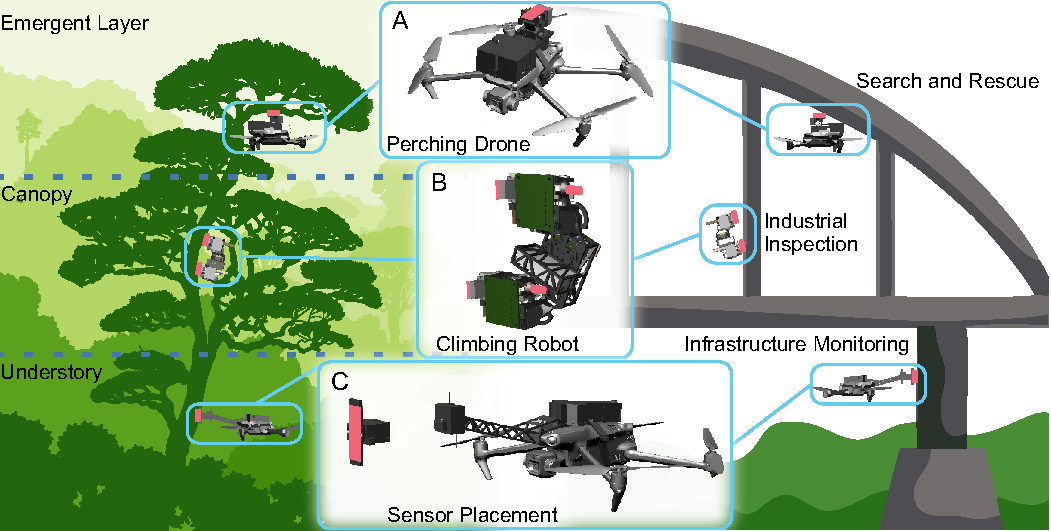
\includegraphics[width=\linewidth]{chapters/papers/SB/figures/fig-1-placeholder/fig-1-placeholder.pdf}
  \caption{Possible applications of biodegradable adhesives for robotic monitoring and inspection in natural and artificial environments: A) perching UAV for long-term monitoring, for instance biodiversity or environmental monitoring, as well as situational awareness in search-and-rescue situations, B) SnailBot, a climbing robot for biodiversity monitoring in tight spaces such as the canopy as well as infrastructure inspection, and C) sensor placement with UAVs for collecting data from otherwise difficult to reach locations.}
  \label{fig:fig1-placeholder}
\end{figure}


High spatial and temporal resolution data is greatly sought after. Examples include environmental and biodiversity monitoring, surveys of infrastructure for predictive maintenance or following the effects of natural disasters, and industrial monitoring. 
Current climate and biodiversity crises \cite{Pereira2024, Weiskopf2024, Pimm2014, Portner2023} underscore the necessity and current lack of comprehensive and scalable environmental and biodiversity monitoring \cite{Gonzalez2023a, McRae2017, Gonzalez2016, Mora2011}. 
Almost a third of all species assessed by the IUCN RedList are deemed to be threatened, yet less than 8\% of the estimated total number of species have been assessed \cite{IUCN2024}.
Biodiversity loss has even been linked to reducing global terrestrial carbon storage \cite{Weiskopf2024}, exacerbating and amplifying carbon emissions and climate change, as well as cascading effects across ecosystems \cite{Rosenberg2019, Ceballos2015}, affecting human social and economic prospects \cite{Frank2024, Portner2023}.

Consistent data collection for infrastructure inspection and industrial monitoring increases in importance with aging infrastructure and reduced human presence in industrial settings. Deteriorating bridges and buildings\cite{Lattanzi2017, Angst2018, Lee2023} raise safety concerns, and increasing automation in more industrial processes \cite{Jurkat2022} reduces physical human presence, expanding the need for scalable remote or autonomous monitoring. 
% TODO: Maybe statistic on how much infrastructure/industrial plants there is, ie how much data is needed



%SM:
% This appetite for data can be only satisfied by the deployment of robots to enable scalable and affordable in-situ data collection. This is relevant especially when accessibility is limited or dangerous. Examples are forests, elevated or partially collapsed infrastructures. 
% In state of the art, we see “universal” strategies for this. Examples are climbing robots, perching robots or deployment of sensors. All these share a common need, adhesion to a substrate. 
% This remain an open challenge, as the current solutions are far from being universal, and instead very specific.  
%=================================Role of Robots=============================================

This demand for data con only be satisfied through the deployment of automatable robots to enable scalable, affordable, and safe in-situ data collection. This is relevant especially when accessibility is limited or dangerous. Examples include forests, elevated structures such as bridges, power lines, off-shore wind farms, or partially collapsed infrastructures following natural disasters. 

%-- forests
% Forests are biodiversity hotspots, home to over half of the world's vertebrate species \cite{Pillay2022} as well as providing essential ecosystem services and climate regulation \cite{Brockerhoff2017}. Tall, remote, and cluttered, they are challenging to access for data collection, even though this data is essential to understand and protect forest functioning and their impact on biodiversity, climate, and overall ecosystem health. Such data is also vital to evaluate the success of strategies aimed at mitigating climate change and reducing biodiversity loss \cite{Gonzalez2023}, especially within the context of the United Nations (UN) Sustainable Development Goals (SDGs). However, concrete data, especially on biodiversity, ecosystems, and climate are still lacking \cite{Goessmann2023} and costly to collect using conventional, mostly manual methods \cite{Cannon2021, UNEnvironment2019}. 
% Developments in robotic environmental monitoring have shown great promise in both accessing challenging locations as well as scaling data collection through automation \cite{LaVigne2022, Charron2020, Kirchgeorg2024, Hamaza, Aucone2023a, Geckeler2022a}.

%Maybe don't go into this much detail...
% Different forest layers have unique challenges for access and require tailored solutions (Figure~\ref{fig:fig1-placeholder}, left). The emergent layer protrudes over the forest canopy and provides potential locations for perching UAVs to conserve battery power while collecting environmental and biodiversity data \cite{Roderick2021, Kirchgeorg2022a, Nguyen2019} The emergent layer and the tops of the canopy can also be accessed from above to collect physical samples through pruning \cite{Charron2020, Krasylenko2023} or swabbing \cite{Kirchgeorg2024, Aucone2023a}. Dense foliage and cluttered branches make the canopy the most difficult area to access, limiting accessibility to probes which can enter from above \cite{Kirchgeorg2024}, launching sensors from further outside \cite{Farinha2020}, or from robots which can remain close to the trunk where vegetation is less dense \cite{Kirchgeorg2023}, including climbing robots \cite{Lam2012, Lam2012a,Dynamics2008c, Liao2020}. The understory is more open which can provide access to UAVs to place sensors against the trunk \cite{Hamaza2020}, collect samples \cite{Krasylenko2023}, or data \cite{Liu2022, Zhou2022}.


% The high and rising human labor costs coupled with the monotonous and repetitive work in often dangerous locations have also driven the demand for more automation in infrastructure and industrial inspection. Elevated infrastructure such as high voltage power lines, bridges, or high-rises as well as off-shore energy infrastructure such as wind farms present unique application opportunities for robots, especially aerial robots \cite{Jiang2023, Paneque2022, Ikeda2017}. In search and rescue scenarios, robots can also explore and stream essential data from partially collapsed buildings to first responders \cite{Zhao2024, Nguyen2023}


Common strategies across multiple application domains include perching robots, climbing robots, and placing sensors. These all show great promise due to expanded accessibility in previously difficult-to-reach ecosystems and locations, as well as providing the possibility to increase efficiency through automation. Specific examples include sensor placement using UAVs for environmental monitoring in forests or industrial inspection \cite{Hamaza, Hamaza2020, Geckeler2022a, Jarvis2018}, climbing robots for biodiversity monitoring \cite{Lam2012} as well as industrial inspection \cite{Hong2022}. Perching UAVs enable longer mission-envelopes by reducing battery consumption \cite{Li2022, Graule2016, Zhang2017a, Hsiao2023}, useful for tasks such as longer-term biodiversity monitoring \cite{Kirchgeorg2023a, Nguyen2019, Roderick2021}, or providing situational awareness in search-and-rescue scenarios \cite{Delmerico2019}.


%SM:
% The quest for high spatial and temporal resolution data is increasing everywhere. Examples are environmental / biodiv monitoring, survey of infrastructures for predictive maintenance or following effects of natural disasters.
% This appetite for data can be only satisfied by the deployment of robots to enable scalable and affordable in-situ data collection. This is relevant especially when accessibility is limited or dangerous. Examples are forests, elevated or partially collapsed infrastructures. 
% In state of the art, we see “universal” strategies for this. Examples are climbing robots, perching robots or deployment of sensors. All these share a common need, adhesion to a substrate. 
% This remain an open challenge, as the current solutions are far from being universal, and instead very specific.  
%=================================Challenge of Adhesion/types of adhesive=============================================
% For multiple uses robots need to adhere to things (sensor placement, climbing robots, perching drones);
% however, most adhesion methods are only good for one type of surface (suction flat, bark, etc)
% glue is good for multiple surfaces, but not environmentally friendly/ leaves residue
% therefore, propose biodegradable adhesive which can attach to multiple different surfaces for env./biodiv monitoring, but also for infrastructure monitoring and industrial inspection.


A critical challenge for all these tasks in the various environments is the method of adhesion to the substrate. This remains an open challenge, as current solutions are usually tailored for a specific task and far from universal.
Different adhesion methods have different behavior depending on the substrate's surface roughness, and different tasks can require different levels of adhesion. This results in unique requirements depending on the substrate and task.
% There are unique requirements depending on the substrate and task, with different adhesion methods having different behavior depending on the substrate's surface roughness, and different tasks requiring different levels of adhesion.


% General Related Works adhesion methods for environmental monitoring (grippers/etc for sensors, physical, magnetic, chemical

% General Adhesion Methods (taken from https://doi.org/10.1142/9789812835772_0003)
% pneumatic (suction cups)
    % -- need to maintain power, smooth non-porous surface
% magnetic
% mechanical clamping/gripping (gripper/microspine)
% electrostatic
    % -- smooth no-conductive surface
% chemical (adhesive) "dry adhesive?" ie gecko skin ??
% hybrid?

% general intro adhesives, why suited (wide range of substrates),
% for environmental monitoring  should be bioegradable since toxic, non decomposible residues in the environment should be avoided.

% \cite{Lim2024} % UV curable adhesive, sensor placement and perching

In  general, adhesion methods can be grouped according to the method of adhesion \cite{LONGO2008, Fang2023}; these are pneumatic \cite{Weston-Dawkes2021}, including suction cups \cite{Li2022, Ge2020, Yoshida2010d, Stuart2019, Liu2020}, magnetic \cite{Hong2022, Zhang2017a,Tache2009a}, mechanical clamping or gripping, also with microspines \cite{Roderick2021, SangbaeKim2005, Dynamics2008c, Askari2024,  Nguyen2019, Kirchgeorg2023a}, electrostatic \cite{Graule2016, Liu2013}, or chemical adhesives \cite{Lee2007}, both "wet" adhesion \cite{Hsiao2023,Osswald2013, Lim2024, Miyake2007} and dry adhesion \cite{Unver2006a, Kim2007, Liu2018a}. Additionally, hybrid approaches can combine multiple mechanisms to improve adhesion performance across different surfaces \cite{Bian2021, Han2021e}.
 
Most adhesion methods work best for a particular type of substrate or surface roughness, with poor performance on others. While magnetic adhesion can provide extremely strong adhesion, it only works on ferromagnetic surfaces. This is widespread in industrial settings but almost nonexistent in natural environments. On the other hand, microspines and gripper-based adhesion work well on rough and unstructured surfaces such as tree bark and branches but fail completely on flat, artificial surfaces such as glass or metal, where pneumatic-based suction cup adhesion is well suited.

% While many approaches try to develop adhesion that is applicable over a wide-range of surfaces, attaching to both smooth surfaces and rough surfaces with the same mechanism is still challenging. This results in solutions tuned and tailored to a specific environment and task, reducing generalizability and requiring costly and inefficient development and optimization for new environments or tasks.
It is still challenging to develop adhesion that is applicable over a wind-range of smooth and rough surfaces, resulting in solutions tuned to a specific environment and task. This reduces generalizability and requires costly and inefficient development and optimization for new environments or tasks.
It can also  be desirable to choose and dimension the level of adhesion; a sensor will require less adhesion strength than a perching UAV, for instance. Chemical adhesives, in particular wet adhesives, provide one of the strongest attachment methods available, also across widely varying substrates \cite{Huang2021}. They are widely utilized in construction and other high-load scenarios. However, a main challenge when utilizing chemical adhesives for robotic use-cases is reversing the attachment mechanism for locomotion or collection. Hot-melt adhesives present a widely available adhesive which can also be easily reversed through the application of heat, and several climbing robots based on this principle have been developed \cite{ROCHAT2011, Wang2013, Osswald2013}. 

%wang2013(ida) no extrusion, surface covered in adhesive

% hybrid adhesion methods exist, but complicated

% wet adhesion works well, but not biodegradabel, ie leaves unwanted residue in industrial environments and potentially toxic ones in natural environments, also not easily reversible usually
% that's why we propose biodegradable adhesive , works well across multiple surfaces also biodegradable. 

However, traditional hot-melt adhesive robots leave behind unwanted residue in the environment, which is problematic since most adhesives use harmful components and are derived from depleting petroleum-based resources \cite{Bassett2016}. Leaving toxic chemicals in natural environments, such as forests for biodiversity or environmental monitoring is unacceptable, as is depositing potential contaminants in industrial settings. To reduce the ecological footprint of robotics it is also desirable to have an adhesive which is fully generated with sustainable and renewable materials to minimize ecological impact.

%=================================Proposed Solution=============================================

% Therefore, we propose the use of gelatin-hydrogels as a completely biodegradable, nontoxic, bioneutral, water-soluble, and even edible adhesive for reversible adhesion across substrates of varying roughness for several robotic monitoring and inspection use cases.

% we showcase the solution in the task of environmental monitoring in forests to access all 3 layres, but necessary in all cases for environmental monitoring e.g. bridge inspection, 

% animal-based glues have been used in xyz \cite[]

% Protein-based glues, such as gelatin, have been used as adhesives since antiquity, usually for woodworking or book-binding \cite{Bye1990}. While still currently used in wood products as an adhesive \cite{Dorr2015, Liu2002}, recently, gelatin-based hydrogels have also been widely investigated for biomedical use \cite{Jaipan2017Gelatin-basedApplications}, pectin-based mixtures for food glue \cite{Moll2022a}, in soft-robotics \cite{Baumgartner2020} or sensing \cite{Hardman2022, Heiden2022, Hardman2021}. 
%then we propose biodegradable adhesive for use in environmental monitoring, suitablie for a variety of different materials of varying roughness, for different uses (perching, climbing robot, sensor placemnt)

%=================================Contributions=============================================
% \cite{Huang2021} => actually uses gelatin hydrogel, but reverse adhesion with electric

% This work proposes the novel use of gelatin-based hydrogels as biodegradable adhesives for use in robotic environmental monitoring.
%main  contributions?
%characterization of hydrogel for use as an adhesiev (ie properties that should be tuned for max. pull-off force
%demonstration on different surface (roughnesses)
% demonstration of utilitiy in three robotic monitoring cases
Therefore, in this work we propose the novel use of gelatin-based hydrogels as a completely biodegradable, biocompatible, renewable, water-soluble, and even edible adhesive for reversible adhesion across substrates of varying roughness for robotic monitoring and inspection use cases. 
% The main contributions of this work are the characterization of the hydrogel for use as an adhesive, investigating the parameters that should be tuned to affect the maximum pull-off force, verification of the maximum pull-off force on different materials with different surface roughnesses, and finally the demonstration of the utility of the adhesive with three robotic monitoring cases, sensor placement with a UAV, UAV perching, and a climbing robot.
Gelatin-based hydrogels present a cheap, easily manufactured adhesive which is easily biodegradable through its water solubility \cite{Hartmann2021}. This presents a viable solution for adhesion in natural environments, where natural rainfall will wash aware any residues, to industrial settings, where residues can also be easily removed with water. To attach to a surface, the hydrogel is heated, pressed against the substrate and cooled. To remove, it is again heated, providing strong, reversible, and controllable adhesion. The adhesive is experimentally characterized to determine optimal usage parameters and their effect on the maximum pull-off force, including the cooling time, the necessary heating temperature, the pressing force against the substrate, and the amount of adhesive used. Additionally, the adhesive is tested on materials with a wide range of surface roughnesses, namely tree bark, concrete brick, medium-density fibreboard (MDF), and glass, as well as sandpaper of different grit, demonstrating the adhesive capabilities of the hydrogel on different surface types. We show that 0.1g of the hydrogel (6mm x 6mm from a 2mm thick sheet) can have a maximum of 45N pull off force, with at least 20N across all surfaces.
The usability of gelatin-based hydrogels for robotic environmental monitoring is showcased through three different applications which enable data collection and access to different environments: sensor placement with a UAV, a perching UAV, and a climbing robot. Using a UAV for sensor placement, sensors can be placed on the trunk of a tree in the understory or for infrastructure monitoring in challenging locations, a perching UAV can provide access to the emergent layer in forests or be used in search-and-rescue scenarios, and a climbing robot can access dense tree canopies or be used in industrial inspection.
%Demonstrated with three different use-cases:
% contribute novel method of robotic environmental monitoring utilizing biodegradable adhesives (first of kind?) demonstrated by utilizing the adhesive for sensor attachment to attach sensors horizontally to tree, deployed by drone
% enables perching of drones for audio/video capture (/monitoring)
% main contributions:
% 1. demonstrate biodegradable adhesive for robotic environmental monitoring
% 2. Characterize biodegradable adhesive (heating temperature, etc)
% 3. showcase three applications for monitoring: sensor placement, perching droen, climbing robot

% Perching is important because xyz, we showcase perching with xyz
% access to canopy is difficult, different approaches suggested, climibing robot feasible, adhesion challenging


\section{Results}
%list in beggining of section what is investiagte,d how supports claim

\subsection{Working Principle}

Figure~\ref{fig:fig-schematic} demonstrates the working principle behind the biodegradable gelatin-hydrogel adhesive. First, the necessary amount of hydrogel, $m$, for the application, is heated to the correct temperature, $T_H$. Then, it is pressed against the substrate with the pressing force $F_P$. The hydrogel is then cooled for time $t_C$, after which it can be loaded, maximally with the maximum pull-off force until detachment $F_M$. To release, the hydrogel is again heated until the connection is broken. Any residue left on the surface can be washed away by water, such as rain in natural environments.

\subsection{Gelatin-based Hydrogel Adhesive}

Protein-based glues, such as gelatin, have been used as adhesives since antiquity, usually for woodworking or book-binding \cite{Bye1990}. While still currently used in wood products as an adhesive \cite{Dorr2015, Liu2002}, recently, gelatin-based hydrogels have also been widely investigated for biomedical use \cite{Jaipan2017}, pectin-based mixtures for food glue \cite{Moll2022a}, in soft-robotics \cite{Baumgartner2020} or sensing \cite{Hardman2022, Heiden2022, Hardman2021}. This work presents the novel use-case of using gelatin-hydrogels as adhesives for robotic monitoring applications. They are well suited for this since they are cheap, easy to source and manufacture, and provides strong adhesion with easy biodegradability and cleanup due to its water solubility \cite{Hartmann2021}.

%should be in Section Working Principle, but pagebreak
\begin{wrapfigure}{r}{0.5\linewidth}
  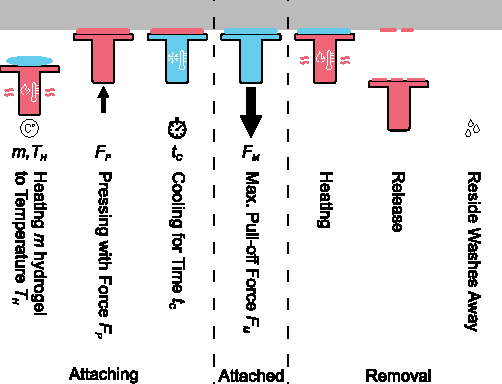
\includegraphics[width=\linewidth]{chapters/papers/SB/figures/fig-schematic/fig-schematic.pdf}
  \caption{Working principle behind gelatin-based hydrogels as adhesives. To attach an object to the substrate, an amount of  hydrogel, $m$, is heated to temperature $T_H$, then pressed against the substrate with force $F_P$. After cooling for time $t_C$, the hydrogel is ready for load-bearing, up to the maximum pull-off force, $F_M$. To remove the object, the hydrogel is again heated, and any remaining residue can be washed away by water.}
  \label{fig:fig-schematic}
\end{wrapfigure}

The gelatin hydrogel used in this work follows the same composition as in \cite{Geckeler2023b}, it is composed of 24 weight percent (wt\%) of gelatin powder (mesh 40 and bloom factor 260), 25.3 wt\% glucose, 32.5 wt\% glycerin (E422, 99.7\%), 14.5 wt\% de-ionized water, and 3.6 wt\% citric acid (E330). The ingredients are mixed under heat, then cast into corresponding moulds. For the hydrogel reservoir glue sticks of the climbing robot SnailBot, it is cast into cylindrical tubes, for all other applications into sheets of 2 mm, which are then laser-cut into 6x6mm squares, the corresponding number of which are used for the specific application as needed. These are then attached to the heating plate for the perching UAV or sensor placement and present a single use.

% For single-use cases, such as the perching UAV or sensor placement, the hydrogel is pre-applied to the mechanism. For this, the hydrogel is manufactured into a sheet, from which the necessary size is laser-cut. For continuous extrusion in the case of the climbing robot, the hydrogel is cast into a cylinder, which is then fed into the mechanism, akin to a hot-glue gun. For details on the hydrogel composition and manufacture, see Section~\ref{subsec:experimental_section-gelatin_hydrogel}.
% The hydrogel is manufactured into a sheet, from which different sizes are cut, resulting in different areas. As expected, higher amounts of glue and surface area result in higher forces. 


\subsection{Gelatin Hydrogel Adhesive Characterization}
\label{subsec:gelatin_charac}

To be useful as an adhesive for any robotic environmental monitoring task, the hydrogel must first be characterized so that the adhesive specifications for a particular task can be achieved. The adhesive properties of the gelatin hydrogel are dependent on several factors, showcased in Figure~\ref{fig:fig-schematic}. These are the cooling time $t_C$, heating temperature $T_H$, pressing force $F_P$, and $m$, the amount of adhesive used. These all affect the maximum pull-off force $F_M$, which is the force needed to detach the object from the surface it is adhered to. This represents the maximum useful load that can be applied to the adhesive, and should be dimensioned according to the application. For instance, a sensor will have lower requirements than an entire perching UAV which must be supported. 
The task-specific necessary maximum pull-off force can also require a different physical design, depending on these parameters. For instance, the cooling time can be adjusted and the design may not require active cooling with a fan and thermoelectric cooling element, but can get by with a passive heatsink.
% This can then also translate to a different physical design, since other parameters, such as the cooling times can also be adjusted and therefore the design may not require active cooling with a fan and Peltier element, but can get by with a simple heatsink. %Thermoelectriccooling element
A benefit of wet adhesives, and the gelatin hydrogel in particular, is the adherence to substrates with different surface roughnesses. To demonstrate this, the maximum pull-off force on different roughness and different materials is tested. Testing of surface roughnesses is done through adhesion to sandpaper of different grit. The different materials tested are glass, brick, bark and MDF. There exist also coarser macroscopic  surface unevenness, in the brick or bark for instance.
% ,  namely glass, brick, bark, and medium-density fibreboard (MDF) are tested, as well as on sandpaper with different roughnesses. 
These tests demonstrate the strong adhesion of the hydrogel despite large variability in the substrate surface roughness and material.

\subsubsection{Adhesive Parameters} % cooling time, heating time, amount of glue, temperature during hetaing time, sample size, shear, pressing force, pressing force ratio 
Differing applications of the adhesive will require different levels of adhesion. 
% To quantify and determine the necessary parameters for a certain level of adhesion we investigate the factors influencing adhesion; the amount of glue used, the temperature to which the hydrogel is heated ($T_H$), the force with which the glue is pressed against the substrate ($F_P$), and the cooling time after attachment ($t_c$).

% \begin{figure}
%   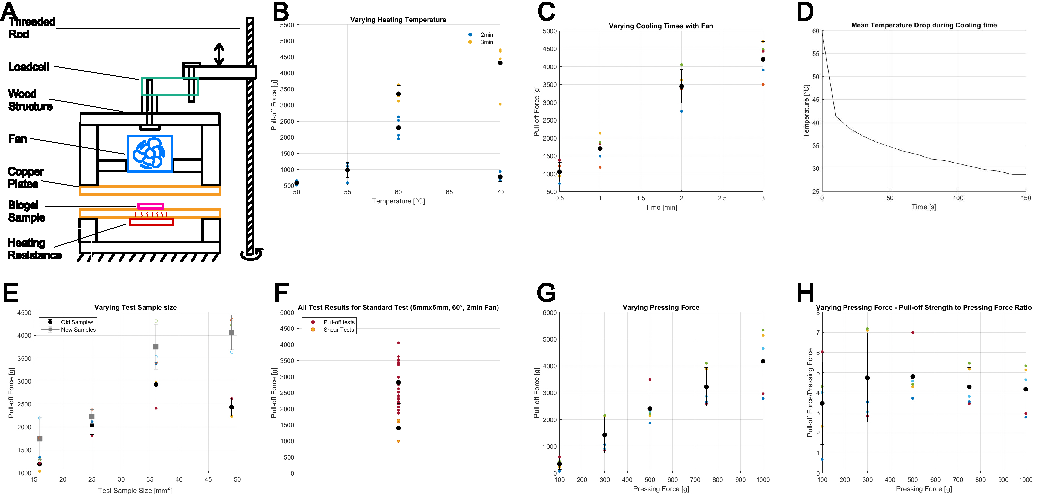
\includegraphics[width=\linewidth]{figures/fig-2-plot-placeholder/fig-2-plot-placeholder.pdf}
%   \caption{Gelatin hydrogel adhesive characterization, pull-off force vs heating temperature, cooling temperature, amount of hydrogel, shear force, and pressing force.}
%   \label{fig:fig2-placeholder}
% \end{figure}

\begin{figure}
\centering
\resizebox{\columnwidth}{0.99\textheight}{%
    \begin{tikzpicture}[ image/.style = {
    text width=0.49\textwidth,
    % text height = 0.25\textwidth,
    inner sep=1pt, outer sep=1pt}, %% default 0,0
    node distance = 3mm and 1mm,  % default 1,1
    ]
    \def\myanchorshift{-0.6cm}
\node [image] (frame1)
{\begin{center}
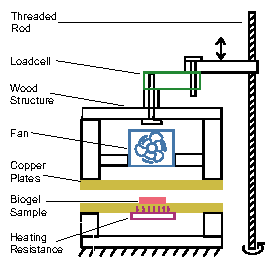
\includegraphics[width=0.7\textwidth]{chapters/papers/SB/figures/fig-2-plot-placeholder/fig-2-plot-placeholder-testsetup.pdf}
\end{center}};
% \node [left=of frame1]{A};
\node[anchor=south west, above left=\myanchorshift] at (frame1.north west) {\large A};
\node [image,right=of frame1] (frame2) 
{\begin{tikzpicture}  [align=center]
  \begin{axis}
    [    
    % boxplot/draw direction = y,
    xmajorgrids,
    minor x tick num=1,
    xminorgrids, 
    ymajorgrids,
    minor y tick num=1, % how many minor ticks to have between major
    yminorgrids,
    % scale=0.9,
    % y dir=reverse, %to have round1 at the top
    % boxplot/box extend=0.4, %control width of boxplot box
    % height=0.5\columnwidth,
    % width= 0.5\columnwidth,
    % xtick={1,2,3,4},
    % xticklabels={0.5,1,2,3},
    % yticklabels={Round 1, Round 2, Round 3, Round 4},
    % xticklabels={VLOS 1, VLOS 2, BVLOS 1, BVLOS 2},
    % xlabel={Time per Collection Attempt (s)},
    % nodes near coords,
    cycle list ={m-blue, m-green, m-red, m-cyan, m-yellow},
    % every axis plot/.append style={thick, fill, fill opacity =0.5},
    % every axis plot/.append style={thick},
    xlabel={Cooling Time (min.)},ylabel={Temperature (C\degree)}]
    \addplot+[line width=1.5pt]table[header=true, col sep=comma] {chapters/papers/SB/figures/fig-2-plot-placeholder/cooling_temperature_curve.csv};
  \end{axis}
  \node at (current axis.north) [anchor=south] {$T_H=60\degree, F_P=4.9N, m=0.1g$};
\end{tikzpicture}

%%%TODO: place median number value? https://tikz.dev/pgfplots/libs-statistics};
\node[anchor=south west, above left=\myanchorshift] at (frame2.north west) {\large B};
\node [image,below=of frame1] (frame3)
    {\begin{tikzpicture}  [align=center]
  \begin{axis}
    [    boxplot/draw direction = y,
    xmajorgrids,
    % minor x tick num=1,
    % xminorgrids, 
    ymajorgrids,
        ymin=0,
    ymax=55,
    minor y tick num=1, % how many minor ticks to have between major
    yminorgrids,
    % scale=0.9,
    % y dir=reverse, %to have round1 at the top
    boxplot/box extend=0.4, %control width of boxplot box
    % height=0.5\columnwidth,
    % width= 0.5\columnwidth,
    xtick={1,2,3,4},
    xticklabels={0.5,1,2,3},
    % yticklabels={Round 1, Round 2, Round 3, Round 4},
    % xticklabels={VLOS 1, VLOS 2, BVLOS 1, BVLOS 2},
    % xlabel={Time per Collection Attempt (s)},
    % nodes near coords,
    cycle list ={m-blue, m-green, m-red, m-cyan, m-yellow},
    every axis plot/.append style={thick, fill, fill opacity =0.5},
    xlabel={$t_c$, Cooling Time (min.) (n=5)},ylabel={$F_M$, Pull-Off Force (N)}]
  \foreach \n in {0,...,3} {
			\addplot+[ boxplot, mark=*, fill, draw=black] table[y index=\n, col sep=comma] {figures/fig-2-plot-placeholder/cooling_time_fan.csv}
      node[left, color=black, fill opacity=1] at (boxplot box cs: \boxplotvalue{median},0)
{\pgfmathprintnumber{\fpeval{round(\boxplotvalue{median},0)}}};
               \pgfplotsset{cycle list shift=-1*(\n+1)} % Goes one style back (offset, not index)
         \addplot+[only marks, mark=*] table[x expr=\n+1.35, y index=\n, col sep=comma] {figures/fig-2-plot-placeholder/cooling_time_fan.csv};
		};
  \end{axis}
      \node at (current axis.north) [anchor=south] {$T_H=60\degree, F_P=4.9N, m=0.1g$};
\end{tikzpicture}

%%%TODO: place median number value? https://tikz.dev/pgfplots/libs-statistics};
\node[anchor=south west, above left=\myanchorshift] at (frame3.north west) {\large C};
\node [image,right=of frame3] (frame4) 
{\begin{tikzpicture}  [align=center]
  \begin{axis}
    [    boxplot/draw direction = y,
    legend pos=north west,
    xmajorgrids,
    % minor x tick num=1,
    % xminorgrids, 
    ymajorgrids,
        ymin=0,
    ymax=55,
    minor y tick num=1, % how many minor ticks to have between major
    yminorgrids,
    % scale=0.9,
    % y dir=reverse, %to have round1 at the top
    boxplot/box extend=0.4, %control width of boxplot box
    % height=0.5\columnwidth,
    % width= 0.5\columnwidth,
    xtick={1,2,3,4},
    % xtick={0,...,10}
    % x tick label as interval,
    xticklabels={50,55,60,70},
    % yticklabels={Round 1, Round 2, Round 3, Round 4},
    % xticklabels={VLOS 1, VLOS 2, BVLOS 1, BVLOS 2},
    % xlabel={Time per Collection Attempt (s)},
    % nodes near coords,
    cycle list ={m-blue, m-green, m-red, m-cyan, m-yellow},
    every axis plot/.append style={thick, fill, fill opacity =0.5},
    xlabel={$T_H$, Heating Temp. (C) (n=5, 2Min 70, 3 Min 60: n=3)},ylabel={$F_M$, Pull-Off Force (N)}]
       \addlegendimage{only marks, mark=square*,mark size=4pt,mark options={color=m-blue}}
\addlegendentry{2 Min. Cooling}
   \addlegendimage{only marks, mark=square*,mark size=4pt,mark options={color=m-red}}
\addlegendentry{3 Min. Cooling}
  \foreach \n in {0,...,3} {
			\addplot+[ boxplot,style=m-blue, mark=*, fill, draw=black] table[y index=\n, col sep=comma] {chapters/papers/SB/figures/fig-2-plot-placeholder/heating_temperature.csv}
      node[left, color=black, fill opacity=1] at (boxplot box cs: \boxplotvalue{median},0)
{\pgfmathprintnumber{\fpeval{round(\boxplotvalue{median},0)}}};
            % \pgfplotsset{cycle list shift=-\n+1} % Goes one style back (offset, not index)
         \addplot+[only marks, mark=*,style=m-blue] table[x expr=\n+1.35, y index=\n, col sep=comma] {chapters/papers/SB/figures/fig-2-plot-placeholder/heating_temperature.csv};
		};
  \foreach \n in {4,...,5} {
  			\addplot+[ boxplot={draw position = \n-1}, style=m-red, mark=*, fill, draw=black] table[y index=\n, col sep=comma] {chapters/papers/SB/figures/fig-2-plot-placeholder/heating_temperature.csv}
        node[left, color=black, fill opacity=1] at (boxplot box cs: \boxplotvalue{median},0)
{\pgfmathprintnumber{\fpeval{round(\boxplotvalue{median},0)}}};
                 \pgfplotsset{cycle list shift=-\n} % Goes one style back (offset, not index)
         \addplot+[only marks, mark=*,style=m-red] table[x expr=(\n-1)+0.35, y index=\n, col sep=comma] {chapters/papers/SB/figures/fig-2-plot-placeholder/heating_temperature.csv};
			% \addplot+[ boxplot={draw position = 4}, style=m-red, mark=*, fill, draw=black] table[y index=5, col sep=comma] {figures/fig-2-plot-placeholder/heating_temperature.csv};
   %             \pgfplotsset{cycle list shift=-5} % Goes one style back (offset, not index)
   %       \addplot+[only marks, mark=*,style=m-red] table[x expr=4.35, y index=5, col sep=comma] {figures/fig-2-plot-placeholder/heating_temperature.csv};
   };
  \end{axis}
  \node at (current axis.north) [anchor=south] {$t_c=2 Min., F_P=4.9N, m=0.1g$};
\end{tikzpicture}

%%%TODO: place median number value? https://tikz.dev/pgfplots/libs-statistics};
\node[anchor=south west, above left=\myanchorshift] at (frame4.north west) {\large D};
\node [image,below=of frame3] (frame5) 
{\begin{tikzpicture}  [align=center]
  \begin{axis}
    [    boxplot/draw direction = y,
    xmajorgrids,
    % minor x tick num=1,
    % xminorgrids, 
    ymajorgrids,
    ymin=0,
    ymax=55,
    minor y tick num=1, % how many minor ticks to have between major
    yminorgrids,
    % scale=0.9,
    % y dir=reverse, %to have round1 at the top
    boxplot/box extend=0.4, %control width of boxplot box
    % height=0.5\columnwidth,
    % width= 0.5\columnwidth,
    xtick={1,2,3,4,5},
    % xticklabels={100,300,500,750,1000},
        xticklabels={0.98, 2.94, 4.90, 7.35, 9.80},
    % yticklabels={Round 1, Round 2, Round 3, Round 4},
    % xticklabels={VLOS 1, VLOS 2, BVLOS 1, BVLOS 2},
    % xlabel={Time per Collection Attempt (s)},
    % nodes near coords,
    cycle list ={m-blue, m-green, m-red, m-cyan, m-yellow},
    every axis plot/.append style={thick, fill, fill opacity =0.5},
    xlabel={$F_P$, Pressing Force (N) (n=5)},ylabel={$F_M$, Pull-Off Force (N)}]
  \foreach \n in {0,...,4} {
			\addplot+[ boxplot, mark=*, fill, draw=black] table[y index=\n, col sep=comma] {figures/fig-2-plot-placeholder/pressing_force.csv}
      node[left, color=black, fill opacity=1] at (boxplot box cs: \boxplotvalue{median},0)
{\pgfmathprintnumber{\fpeval{round(\boxplotvalue{median},0)}}};
                  \pgfplotsset{cycle list shift=-1*(\n+1)} % Goes one style back (offset, not index)
         \addplot+[only marks, mark=*] table[x expr=\n+1.35, y index=\n, col sep=comma] {figures/fig-2-plot-placeholder/pressing_force.csv};
		};
  \end{axis}
  \node at (current axis.north) [anchor=south] {$t_c=2 Min., T_H=60\degree, m=0.1g$};
\end{tikzpicture}

%%%TODO: place median number value? https://tikz.dev/pgfplots/libs-statistics};
\node[anchor=south west, above left=\myanchorshift] at (frame5.north west) {\large E};
\node [image,right=of frame5] (frame6) 
{\begin{tikzpicture}  [align=center]
  \begin{axis}
    [    boxplot/draw direction = y,
    xmajorgrids,
    % minor x tick num=1,
    % xminorgrids, 
    ymajorgrids,
    minor y tick num=1, % how many minor ticks to have between major
    yminorgrids,
    % scale=0.9,
    % y dir=reverse, %to have round1 at the top
    boxplot/box extend=0.4, %control width of boxplot box
    % height=0.5\columnwidth,
    % width= 0.5\columnwidth,
    xtick={1,2,3,4,5},
    % xticklabels={100,300,500,750,1000},
    xticklabels={0.98, 2.94, 4.90, 7.35, 9.80},
    % yticklabels={Round 1, Round 2, Round 3, Round 4},
    % xticklabels={VLOS 1, VLOS 2, BVLOS 1, BVLOS 2},
    % xlabel={Time per Collection Attempt (s)},
    % nodes near coords,
    cycle list ={m-blue, m-green, m-red, m-cyan, m-yellow},
    every axis plot/.append style={thick, fill, fill opacity =0.5},
    xlabel={$F_P$, Pressing Force (N) (n=5)},ylabel={Ratio Pull-Off/Pressing Force}]
  \foreach \n in {0,...,4} {
			\addplot+[ boxplot, mark=*, fill, draw=black] table[y index=\n, col sep=comma] {chapters/papers/SB/figures/fig-2-plot-placeholder/pressing_force_ratio.csv}
      node[left, color=black, fill opacity=1] at (boxplot box cs: \boxplotvalue{median},0)
{\pgfmathprintnumber{\fpeval{round(\boxplotvalue{median},0)}}};
                  \pgfplotsset{cycle list shift=-1*(\n+1)} % Goes one style back (offset, not index)
         \addplot+[only marks, mark=*] table[x expr=\n+1.35, y index=\n, col sep=comma] {chapters/papers/SB/figures/fig-2-plot-placeholder/pressing_force_ratio.csv};
		};
  \end{axis}
  \node at (current axis.north) [anchor=south] {$t_c=2 Min., T_H=60\degree, m=0.1g$};
\end{tikzpicture}

%%%TODO: place median number value? https://tikz.dev/pgfplots/libs-statistics};
\node[anchor=south west, above left=\myanchorshift] at (frame6.north west) {\large F};
\node [image,below=of frame5] (frame7) 
{\begin{tikzpicture}  [align=center]
  \begin{axis}
    [    boxplot/draw direction = y,
    xmajorgrids,
    % minor x tick num=1,
    % xminorgrids, 
    ymajorgrids,
        ymin=0,
    ymax=55,
    minor y tick num=1, % how many minor ticks to have between major
    yminorgrids,
    % scale=0.9,
    % y dir=reverse, %to have round1 at the top
    boxplot/box extend=0.4, %control width of boxplot box
    % height=0.5\columnwidth,
    % width= 0.5\columnwidth,
    xtick={1,2,3,4},
    % xticklabels={0.05/16,0.07/25,0.10/36,0.14/49},
    xticklabels={0.05,0.07,0.10,0.14},
    % yticklabels={Round 1, Round 2, Round 3, Round 4},
    % xticklabels={VLOS 1, VLOS 2, BVLOS 1, BVLOS 2},
    % xlabel={Time per Collection Attempt (s)},
    % nodes near coords,
    cycle list ={m-blue, m-green, m-red, m-cyan, m-yellow},
    every axis plot/.append style={thick, fill, fill opacity =0.5},
    xlabel={$m$, Biogel Sample Amount ($g$) (n=3)},ylabel={$F_M$, Pull-Off Force (N)}]
  \foreach \n in {0,...,3} {
			\addplot+[ boxplot, mark=*, fill, draw=black] table[y index=\n, col sep=comma] {chapters/papers/SB/figures/fig-2-plot-placeholder/biogel_sample_size.csv}
      node[left, color=black, fill opacity=1] at (boxplot box cs: \boxplotvalue{median},0)
{\pgfmathprintnumber{\fpeval{round(\boxplotvalue{median},0)}}};
                     \pgfplotsset{cycle list shift=-1*(\n+1)} % Goes one style back (offset, not index)
         \addplot+[only marks, mark=*] table[x expr=\n+1.35, y index=\n, col sep=comma] {chapters/papers/SB/figures/fig-2-plot-placeholder/biogel_sample_size.csv};
		};
  \end{axis}
  \node at (current axis.north) [anchor=south] {$t_c=2 Min., T_H=60\degree, F_P=4.9N$};
\end{tikzpicture}

%%%TODO: place median number value? https://tikz.dev/pgfplots/libs-statistics};
\node[anchor=south west, above left=\myanchorshift] at (frame7.north west) {\large G};
\node [image,right=of frame7] (frame8) 
{\begin{tikzpicture}  [align=center]
  \begin{axis}
    [    boxplot/draw direction = y,
    % xmajorgrids,
    % minor x tick num=1,
    % xminorgrids, 
    ymajorgrids,
        ymin=0,
    ymax=55,
    minor y tick num=1, % how many minor ticks to have between major
    yminorgrids,
    % scale=0.9,
    % y dir=reverse, %to have round1 at the top
    boxplot/box extend=0.4, %control width of boxplot box
    % height=0.5\columnwidth,
    % width= 0.5\columnwidth,
    xtick={1,2},
    xticklabels={Normal, Shear},
    % yticklabels={Round 1, Round 2, Round 3, Round 4},
    % xticklabels={VLOS 1, VLOS 2, BVLOS 1, BVLOS 2},
    % xlabel={Time per Collection Attempt (s)},
    % nodes near coords,
    cycle list ={m-blue, m-green, m-red, m-cyan, m-yellow},
    every axis plot/.append style={thick, fill, fill opacity =0.5},
    xlabel={Normal vs Shear (n=5)},ylabel={$F_M$, Pull-Off Force (N)}]
  % \foreach \n in {0,...,1} {
			\addplot+[ boxplot, mark=*, fill, draw=black] table[y index=0, col sep=comma] {figures/fig-2-plot-placeholder/shear_force.csv}
      node[left, color=black, fill opacity=1] at (boxplot box cs: \boxplotvalue{median},0)
{\pgfmathprintnumber{\fpeval{round(\boxplotvalue{median},0)}}};
        \pgfplotsset{cycle list shift=-1} 
         \addplot+[only marks, mark=*, ] table[x expr=1.35, y index=0, col sep=comma] {figures/fig-2-plot-placeholder/shear_force.csv};
         \addplot+[ boxplot, mark=*, fill, style=m-red,draw=black] table[y index=1, col sep=comma] {figures/fig-2-plot-placeholder/shear_force.csv}
            node[left, color=black, fill opacity=1] at (boxplot box cs: \boxplotvalue{median},0)
{\pgfmathprintnumber{\fpeval{round(\boxplotvalue{median},0)}}};
         \pgfplotsset{cycle list shift=-2} % Goes one style back (offset, not index)
         \addplot+[only marks, mark=*, style=m-red] table[x expr=2.35, y index=1, col sep=comma] {figures/fig-2-plot-placeholder/shear_force.csv};
		% };
  \end{axis}
  \node at (current axis.north) [anchor=south] {$t_c=2 Min., T_H=60\degree, F_P=4.9N, m=0.1g$};
\end{tikzpicture}

%%%TODO: place median number value? https://tikz.dev/pgfplots/libs-statistics};
\node[anchor=south west, above left=\myanchorshift] at (frame8.north west) {\large H};
\end{tikzpicture}
}
  \caption{Plots showing characterization of the factors affecting adhesion of the biodegradable gelatin-hydrogel.}
  \label{fig:fig-2-plots-placeholder}

\end{figure}

Figure~\ref{fig:fig-2-plots-placeholder} shows the maximum pull-off force ($F_M$) as a function of the different parameters affecting adhesion. Figure~\ref{fig:fig-2-plots-placeholder}A shows the test setup. A certain amount of hydrogel ($m$, Figure~\ref{fig:fig-2-plots-placeholder}G) is placed on top of a fixed copper plate, which is above a heating resistance wire to heat the hydrogel to a specific temperature ($T_H$, Figure~\ref{fig:fig-2-plots-placeholder}D) and initiate the adhesion process. A second movable copper plate is lowered, pressing against the adhesive with a certain force ($F_P$, Figure~\ref{fig:fig-2-plots-placeholder}E,F), measured by a loadcell. 
% First, the hydrogel is heated to the specified temperature, sandwiched between the plates, then cooled for either two or three minutes. The movable plate is raised and the maximum force until separation is measured. 
A fan and heatsink on the upper copper plate provides active cooling ($t_c$, Figure~\ref{fig:fig-2-plots-placeholder}B,C) to complete adhesion. The movable plate is then raised and the maximum force until separation is measured ($F_M$).  For a detailed description of the components, see the Experimental Section, Section~\ref{sec:experimental_section}.% maybe in experimental seciton
 The standard settings for each test, unless otherwise specified is heating 0.1g of hydrogel to 60\degree\, pressing with 4.9 N, and then cooling for 2 minutes.

%cooling time
To determine how long to wait for the hydrogel to cool, the pull-off force was measured at varying cooling times (Figure~\ref{fig:fig-2-plots-placeholder}C).
% A fan blows air onto the movable copper plate to expedite cooling.
The plot reflects a strong trend of stronger-pull-of forces with longer cooling times, albeit with diminishing returns. 
%temperature during heating time,
This can be seen in Figure~\ref{fig:fig1-placeholder}B, which shows the temperature development during cooling for one sample. Most of the temperature drops within the first 30 seconds, with the rate of cooling decreasing asymptotically. 
Interesting to note is that while cooling for two or three minutes results in a difference of only 2\degree C, there is disproportionally large improvement in the pull-off force, indicating either a high sensitivity to temperature, or the contribution of other factors.
Higher pull-off forces are of course desirable, but must be weighed against the additional cost of time.
Under these considerations, a cooling time of two minutes was selected for standard applications.
% Under this consideration, and desiring to minimize waiting times and with the previously measured sufficient pull-off forces at 60\degree, a cooling time of two minutes was selected for standard applications. 
%TODO Check whether diminishing returns (ie plot delta, change in temperature per time, ie difference 1-2 MIN vs 2-3 min), maybe line plot with additional axis on right? => derivative of trendline

% Heating Temperature,
Figure~\ref{fig:fig-2-plots-placeholder}D shows the effect of varying the maximum heating temperature ($T_H$) on the pull-off force ($F_M$). The graph indicates that longer cooling times (3 minutes, in red) benefit the adhesion force, with the maximum pull-off force of more than 4kg achieved at 70\degree\, heating followed by three minutes of cooling. However, the trade-off between the additional time needed to heat first to 70\degree, then cool for another minute must be considered against  the already impressive (and for two minutes cooling, better) performance at 60\degree. Since for the UAV tasks the pull-off force is already sufficient and flight time is critical, heating to 60\degree\, was chosen as the standard for all other tests.

%pressing force,
%pressing force ratio(??)
Another parameter of interest is the force used to press the adhesive between the object and the substrate. Higher pressing force will result in a more uniform and further spreading of the adhesive, as well as increased surface area. Indeed, as shown in Figure~\ref{fig:fig-2-plots-placeholder}E, we see that for higher pressing forces, a larger pull-off force is measured. Figure~\ref{fig:fig-2-plots-placeholder}F shows the ratio of the pull-off force to pressing force, in other words how much the pull-off force increases in relation to how much the pressing force has increased. This shows that despite the seemingly linear relationship in Figure~\ref{fig:fig1-placeholder}E, the ratio actually plateaus and decreases slightly, since the physical limits of increasing pull-off force with increasing pressing force are approached. Higher pressing force will spread the hydrogel thinner and more evenly, increasing pull-off force, but it is to be expected that this change will eventually plateau once the glue has spread across the entire contact area and has reached optimal thickness. Since pressing force can be difficult to generate, for instance, requiring larger and more expensive motors in a climbing robot, the point before diminishing returns can be selected (5N of pressing force), and any potentially still required pull-off force can then be compensated by adjusting the other parameters.
%300-500g of pressing force

%amount of glue/sample size,
The amount of glue also plays an important role when considering the adhesive strength.  Increased surface area promotes adhesion; however too much glue at a fixed pressing force will also increase thickness of the glue, which will reduce the relative increase in adhesion. Figure~\ref{fig:fig-2-plots-placeholder}G shows the effect on pull-off strength when increasing hydrogel sample sizes, from 0.05, 0.07, 0.10, and 0.14g. The hydrogel is prepared in sheets with 2mm thickness, therefore this corresponds to areas of 4x4mm (16mm$^2$), 5x5mm (25mm$^2$), 6x6mm (36mm$^2$), and 7x7mm (49mm$^2$). The density of the hydrogel is around 1.4 g/cm$^3$. Within this range, increasing the amount of hydrogel consistently increases the pull-off force, indicating that this value should be chosen according to the application. For the tests, 0.1g was chosen as the best adhesive amount/pull-off force trade-off.
%amount of glue, newer sample older -> probably just show new samples, adding old samples will just be confusing

%shear
All previous tests were as a function of the pull-off force in the normal direction. This is accurate for the perching UAV on horizontal surfaces, and the climbing robot when climbing upside-down. For sensor placement or climbing in other configurations, the shear force will should also be considered. Figure~\ref{fig:fig-2-plots-placeholder}H shows the shear forces of the adhesive, compared with the normal forces. As expected, the maximum pull-off forces in shear are less than those in the normal direction, however still quite resilient with an average of 14N or 1.5 kg of supported weight. This provides useful information, complementing the previous parameters to determine the appropriate dimensioning of the hydrogel for a particular use-case, including shear cases.


\subsubsection{Surface Tests} % pull-off force vs different materials
\label{subsec:surface_tests}
\begin{wrapfigure}{r}{0.5\linewidth}
  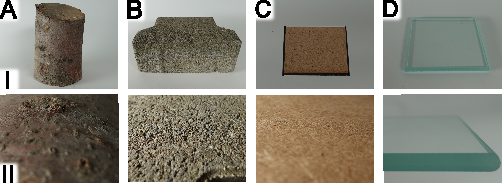
\includegraphics[width=\linewidth]{chapters/papers/SB/figures/fig-3-surfaces-placeholder/fig-3-surfaces.pdf}
  \caption{Different materials used in the maximum pull-off force tests (I), with close-ups showcasing the surface roughness (II). A) Bark, B) Concrete brick, C) MDF, D) Glass}
  \label{fig:fig3-placeholder}
\end{wrapfigure}

To ensure adhesion across a variety of substrates for monitoring applications in different environments, the performance of the adhesive on surfaces with varying degrees of surface roughness is investigated. While most adhesion methods are only suited for specific surfaces (e.g. suction cups for smooth surfaces or microspines for rough surfaces), the gelatin hydrogel showcases similar performance on varying surface roughness, and demonstrates strong adhesion of at least 20N even on materials with very different roughness (glass to tree bark).

\begin{figure}
\centering
% \resizebox{\columnwidth}{0.99\textheight}{%
    \begin{tikzpicture}[ image/.style = {text width=0.49\textwidth,
    % text height = 0.3\textwidth,
    inner sep=1pt, outer sep=1pt}, %% default 0,0
    node distance = 1mm and 1mm,  % default 1,1
    ]
    \def\myanchorshift{-0.6cm}
\node [image] (frame1)
{\begin{tikzpicture}  [align=center]
  \begin{axis}
    [boxplot/draw direction = y,
    % xmajorgrids,
    % minor x tick num=1,
    % xminorgrids, 
    ymajorgrids,
    ymin=0,
    ymax=70,
    minor y tick num=1, % how many minor ticks to have between major
    yminorgrids,
    % scale=0.9,
    % y dir=reverse, %to have round1 at the top
    boxplot/box extend=0.4, %control width of boxplot box
    % height=0.5\columnwidth,
    % width= 0.5\columnwidth,
    xtick={1,2,3},
    % xticklabels={100,300,500,750,1000},
    xticklabels={K80,K240,K320},
    % yticklabels={Round 1, Round 2, Round 3, Round 4},
    % xticklabels={VLOS 1, VLOS 2, BVLOS 1, BVLOS 2},
    % xlabel={Time per Collection Attempt (s)},
    % nodes near coords,
    cycle list ={m-blue, m-green, m-red, m-cyan, m-yellow},
    every axis plot/.append style={thick, fill, fill opacity =0.5},
    xlabel={Sandpaper Grit (K80,K240: n=5, K320: n=4)},ylabel={$F_M$, Pull-Off Force (N)}]
  \foreach \n in {0,...,2} {
			\addplot+[ boxplot, mark=*, fill, draw=black] table[y index=\n, col sep=comma] {chapters/papers/SB/figures/fig-3-surfaces-placeholder/surface_roughness.csv}
   node[left, color=black, fill opacity=1] at (boxplot box cs: \boxplotvalue{median},0)
{\pgfmathprintnumber{\fpeval{round(\boxplotvalue{median},0)}}};
         \pgfplotsset{cycle list shift=-1*(\n+1)} % Goes one style back (offset, not index)
         \addplot+[only marks, mark=*] table[x expr=\n+1.35, y index=\n, col sep=comma] {chapters/papers/SB/figures/fig-3-surfaces-placeholder/surface_roughness.csv};
         % \node at (axis cs:1, 2) [anchor=east] {Median};
		};
%   \pgfplotsinvokeforeach {1,2,3} { % Change numbers to the total number of boxplots/groups
%     \node at (axis cs:#1-0.25,\pgfplotsboxplotvalue{median}) [anchor=east, font=\small] {\pgfmathprintnumber{\pgfplotsboxplotvalue{median}}};
% };

  % \node at (axis cs:0.8,25) [anchor=east, font=\small] {25};
  % \node at (axis cs:0.75,\pgfplotsboxplotvalue{median}) [anchor=east, font=\small] {\pgfmathprintnumber{\pgfplotsboxplotvalue{median}}};
        % node[right] at (boxplot box cs: \boxplotvalue{average}, .5) {\pgfmathprintnumber{\boxplotvalue{average}}}
           \draw[-{Latex[round]}, thick] (axis cs:1,4) -- (axis cs:3,4) node[midway, above] {Increasing Smoothness};
  \end{axis}
    \node at (current axis.north) [anchor=south] {$t_c=2 Min., T_H=60\degree, F_P=4.9N, m=0.1g$};
\end{tikzpicture}

%%%TODO: place median number value? https://tikz.dev/pgfplots/libs-statistics};
% \node [above left=of frame1] {A}; %  at (-4,2)
\node[anchor=south west, above left=\myanchorshift] at (frame1.north west) {\large A};
\node [image,right=of frame1] (frame2) 
{\begin{tikzpicture}  [align=center]
  \begin{axis}
    [boxplot/draw direction = y,
    % xmajorgrids,
    % minor x tick num=1,
    % xminorgrids, 
    ymajorgrids,
    ymin=0,
    ymax=70,
    minor y tick num=1, % how many minor ticks to have between major
    yminorgrids,
    % scale=0.9,
    % y dir=reverse, %to have round1 at the top
    boxplot/box extend=0.4, %control width of boxplot box
    % height=0.5\columnwidth,
    % width= 0.5\columnwidth,
    xtick={1,2,3,4},
    % xticklabels={100,300,500,750,1000},
    xticklabels={Bark, Brick, MDF, Glass},
    % yticklabels={Round 1, Round 2, Round 3, Round 4},
    % xticklabels={VLOS 1, VLOS 2, BVLOS 1, BVLOS 2},
    % xlabel={Time per Collection Attempt (s)},
    % nodes near coords,
    cycle list ={m-blue, m-green, m-red, m-cyan, m-yellow},
    every axis plot/.append style={thick, fill, fill opacity =0.5},
    xlabel={Material (n=5)},ylabel={$F_M$, Pull-Off Force (N) (n=5)}]
  \foreach \n in {0,...,3} {
			\addplot+[ boxplot, mark=*, fill, draw=black] table[y index=\n, col sep=comma] {figures/fig-3-surfaces-placeholder/surface_materials.csv}
   %show median value
      node[left, color=black, fill opacity=1] at (boxplot box cs: \boxplotvalue{median},0)
{\pgfmathprintnumber{\fpeval{round(\boxplotvalue{median},0)}}};
            \pgfplotsset{cycle list shift=-1*(\n+1)} % Goes one style back (offset, not index)
         \addplot+[only marks, mark=*] table[x expr=\n+1.35, y index=\n, col sep=comma] {figures/fig-3-surfaces-placeholder/surface_materials.csv};
		};
   \draw[-{Latex[round]}, thick] (axis cs:1,4) -- (axis cs:4,4) node[midway, above] {Increasing Smoothness};
  \end{axis}
    \node at (current axis.north) [anchor=south] {$t_c=2 Min., T_H=60\degree, F_P=4.9N, m=0.1g$};
\end{tikzpicture}

%%%TODO: place median number value? https://tikz.dev/pgfplots/libs-statistics};
% \node [above left=of frame2] {B}; %  at (-4,2)
\node[anchor=south west, above left=\myanchorshift] at (frame2.north west) {\large B};
\end{tikzpicture}
% }
  \caption{Maximum pull-off force with different surface roughnesses (A) and materials (B).}
  \label{fig:fig-plot-surfaces}

\end{figure}

%actually 103-109mm in diameter
%roughness from https://astropak.com/surface-roughness-average-ra/
The test-setup used to measure the surface roughness tests is similar to the test-setup for the maximum pull-off forces (Figure~\ref{fig:fig-2-plots-placeholder}A), except that it is modified to hold different materials instead of a second copper plate. As in the previous test, 0.1 g of hydrogel were used for each test. The different materials used can be seen in Figure~\ref{fig:fig3-placeholder}, these include tree bark from a trunk segment (with curvature) around 100mm in diameter, a concrete brick, MDF, and window glass. Figure~\ref{fig:fig-plot-surfaces}A, shows the pull-off force with three different sandpaper grit, K80, K240, and K320 (surface roughnesses 1.8$\micro$m , 0.38$\micro$m, and 0.30$\micro$m, respectively). Larger K indicates smoother sandpaper, with K80 being the roughest. The hydrogel adhesive performs comparably, slighly worse for K80 and with no direct discernible trend between K240 and K320. The pull-off force with different materials can be seen in Figure~\ref{fig:fig-plot-surfaces}B. While there is a trend towards higher pull-off forces with smoother surfaces, even with the lowest pull-of force of the bark, the average pull-off force is still 20N. Since the bark (Figure~\ref{fig:fig3-placeholder}A) is actually a part of a small tree trunk there is quite some curvature, with large asperities on the surface. Since the copper plate does not conform to the curvature, there is correspondingly less surface area in contact with the adhesive, which also reduces the pull-off force. These materials not only have different surface roughnesses, but also macroscopic deviations, such as knots and nubs in the wood and small pits in the brick (Figure~\ref{fig:fig3-placeholder}A-II, B-II). Overall, these tests show that the gelatin hydrogel performs well across materials with wide-ranging surface roughnesses, providing adhesion for multiple potential use cases in many different environments. 
% supports the fact that the glue works well on materials with various surface roughnesss


\subsubsection{Water Solubility}
\begin{wrapfigure}{r}{0.5\linewidth}
  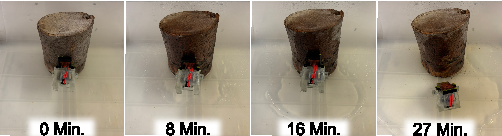
\includegraphics[width=\linewidth]{figures/fig-water-solubility/fig-water-solubility.pdf}
  \caption{Gelatin-hydrogel water solubility removes sensor attached to trunk under simulated rainfall.}
  \label{fig:fig-water-solubility}
\end{wrapfigure}
Besides being biocompatible, renewable, and biodegradable, the gelatin hydrogel is also water-soluble. This facilitates automatic residue removal from natural surfaces through rain and also easy removal in artificial environments through water. This also provides a useful method for removing sensors attached to trees. For instance, to investigate water-based forest stresses, the sensor can be attached to a tree in a forest during drought, and then be re-collected after rain. The rainwater will dissolve attachment, and the sensor-box can be easily collected from the forest floor, where Bluetooth and WiFi available on the sensor-board can be used to aid localization. 
The hydrogel dissolving in water can be seen in \cite{Geckeler2023b}. A demonstration showcasing the sensor removal using simulated rainfall can be seen in Figure~\ref{fig:fig-water-solubility}. This involves the sensor from Section~\ref{subsec:sensor_attachment}. The sensor is attached to tree bark, and falls off after the intermittent spraying application of 260 ml of water over 27 minutes (Figure~\ref{fig:fig-water-solubility}). 
%257ml/water, 27 min.
% %% TODO: should also have picture/image of this




\subsection{Sensor Attachment with UAV}
\label{subsec:sensor_attachment}

Sensors can monitor and collect data without continuous physical human or robot presence. This is especially useful for longer-term monitoring in difficult-to access environments, such as forests or industrial settings \cite{Geckeler2022a, Hamaza, Jarvis2018}. A multitude of distributed sensors can also be used for IoT or mesh networks over larger areas. In such environments, and at at such scales, it can be beneficial to place and attach sensors using UAVs. 
However, few works have looked at the method of attachment, usually simplifying the use-cases to magnets or using double-sided tape. This approach limits the applicability and also introduces challenges when recollecting the sensor. We present the use of a biodegradable gelatin hydrogel as an adhesive for attaching sensors (Figure~\ref{fig:fig4-placeholder}). By using gelatin hydrogel as an adhesive, the sensor can be strongly but reversibly attached to various substrates with different surface roughnesses, from tree bark to glass.

% Figure left CAD/pic render of mechanism (drone shaded out), right stills from video of procedure, approach, pushing, detatchment
\begin{figure}
  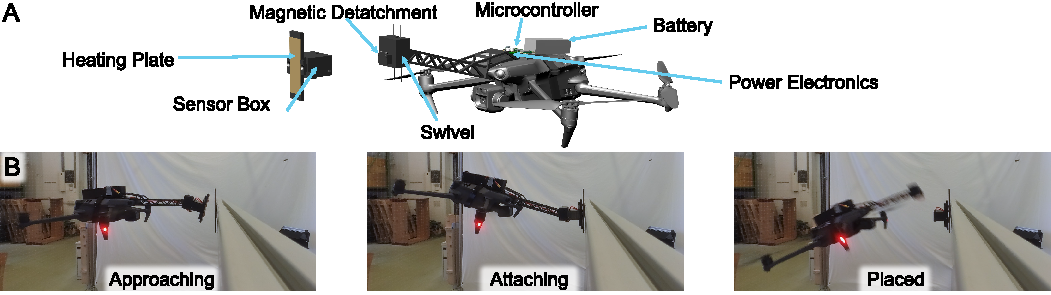
\includegraphics[width=\linewidth]{chapters/papers/SB/figures/fig-4-sensor-placement-placeholder/fig-4-sensor-placement-placeholder.pdf}
  \caption{Sensor Placement with a UAV. A) showcases the different components of the sensor placing payload on the UAV, the sensor box has a heating plate with the hydrogel adhesive, which has a magnetic mechanical and electrical connection to the UAV for heating the plate. A swivel joint de-couples the UAV pitch from the sensor box orientation and facilitates better alignment. B) showcases the attachment process, the UAV heats the hydrogel, attaches the sensor and pitches forward, maintaining force and contact until the adhesive is sufficiently cooled, and pitches back which shears the magnetic connection and detaches the sensor.}
  \label{fig:fig4-placeholder}
\end{figure}

% We present the use of a biodegradable gelatin hydrogel as an adhesive for attaching sensors (Figure~\ref{fig:fig4-placeholder}).
The hydrogel is pre-applied to a copper heating plate. Behind this is the sensor box, which houses the sensing components, in our case temperature, humidity, and light for microclimate measurements. Behind the heating plate is a resistive heating element, which heats the adhesive to the required temperature for adhesion. It is powered through a magnetic mechanical and electrical connection which also attaches the box to the boom on the UAV during flight. A swivel joint behind the magnetic attachments allows de-coupling of the pitch of the UAV with the sensor attitude, permitting easier alignment and transmission of force. A microcontroller controls the heating through WiFi, and power electronics regulate the voltage from a separate onboard battery which powers the payload. A separate battery is used to provide modularity and easy transferability to other platforms. This weight can of course be saved if the payload is integrated to use power directly from the UAV. For a detailed component list, see the Experimental Section~\ref{subsec:experimental_sensor_placing}. 

Figure~\ref{fig:fig4-placeholder}B shows the three stages of sensor attachment with the UAV. First, the UAV aligns and approaches the target, at which point the heating cycle begins and the heating plate is heated for a specific amount of time to reach 60\degree C. If the time to target is known, the heating and cooling can be started beforehand to ensure optimal temperature for attachment without having to spend additional time waiting for the heating cycle to complete. After this, during the attaching phase, the UAV makes contact and continues to pitch forward to provide the necessary pressing force to attach the sensor to the substrate. For lighter weights such as the sensor, pressing only a few seconds with the right temperature is enough to attach the sensor without having to fully wait for cooling to complete (see Supplementary Video S1 for the sensor placement procedure). At this stage the swivel joint permits alignment of the sensor box to the surface while the UAV is still pitching. The UAV maintains contact until the adhesive is sufficiently cooled. To reduce weight and the number of electronic components bundled with the detaching sensor, passive cooling is used. Due to the light sensor weight even after a few seconds of pressing the glue has cooled enough to sustain the weight of the sensor. In the final stage the UAV detaches from the sensor by pitching back, at which point the magnetic connection detaches through the shear force and the sensor is placed and attached. 

Currently, the sensor is designed to remain attached to a tree until the next rainfall. For instance, to investigate water-based forest stresses, the sensor can be attached to a tree in a forest during drought, and then be re-collected after rain. The water solubility of the hydrogel and the possibility of using this for sensor removal can be seen in Figure~\ref{fig:fig-water-solubility}.
% The rainwater will dissolve attachment, and the sensor-box can be easily collected from the forest floor., where Bluetooth and WiFi available on the sensor-board can be used to aid localization.
% A demonstration showcasing the hydrogel dissolving in water can be seen in \cite{Geckeler2023b}.

% to investigate water-based forest stresses, the sensor can be attached to a tree in a forest during drought, and then be re-collected after rain. The rainwater will dissolve attachment, and the sensor-box can be easily collected from the forest floor, where Bluetooth and WiFi available on the sensor-board can be used to aid localization. 
% % A demonstration showcasing the sensor removal using simulated precipitation can be seen in Figure ref{TODO}. After the application of XX ml of water, the sensor falls off within XX minutes.
% A demonstration showcasing the hydrogel dissolving in water can be seen in \cite{Geckeler2023b}.


\subsection{UAV Perching}
\label{subsec:UAV_perching}
% Related Works specific Perching
% Gripper-based  \cite{Kirchgeorg2023a}
% Microspine-based \cite{Nguyen2019}
% Magnet based  spidermav
% adhesive based ~~

The utility of UAV perching has been investigated for a diverse multitude of use cases, from environmental monitoring in forests to search and rescue situations. Attachment for perching UAVs range from pneumatic suction\cite{Li2022, Liu2020}, microspine grapples \cite{Nguyen2019}, microspine grippers \cite{Kirchgeorg2023a}, electrostatic adhesion \cite{Graule2016}, bird-inspired grippers \cite{Roderick2021}, magnetic adhesion \cite{Zhang2017a}, or adhesives \cite{Hsiao2023}.
To enable reversible adhesion without problematic residue across a variety of substrates, we propose a UAV perching mechanism utilizing biodegradable gelatin hydrogel adhesives (Figure~\ref{fig:fig5-placeholder}A).


%Proposed Mechanism 
%Figure with stills from video (ie approaching, pushing, perched, spinning, take-off next to CAD/pic render of mechanism
\begin{figure}
  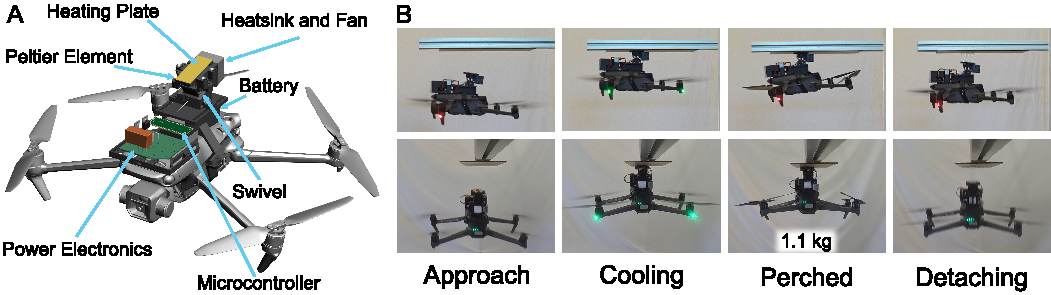
\includegraphics[width=\linewidth]{chapters/papers/SB/figures/fig-5-perching-placeholder/fig-5-perching-placeholder.pdf}
  \caption{UAV Perching: A) CAD Render of perching mechanism with components. B) Perching Sequence: the UAV approaches the target after heating the hydrogel for 30 seconds(Approach), pushes against it and cools the hydrogel (Cooling) for 3 minutes, at which point the UAV (1.1 kg) is perched and the motors can be switched off. To detach, the hydrogel is again heated, and the UAV can re-engage motors to resume flight.}
  \label{fig:fig5-placeholder}
\end{figure}
Similar to the sensor attachment mechanism in Section~\ref{subsec:sensor_attachment}, the adhesive is pre-applied to the heating plate, which is now actively cooled to provide maximal adhesive performance, since the UAV (1.1kg) is quite a bit heavier than the sensor (64g, see Table~\ref{tab:weight}). Beneath the heating plate is a thermoelectric (Peltier) element which can heat or cool the heating plate depending on the polarity of the applied current, attached to a heatsink and fan to cool the other side of the element. This is then attached to the UAV via a swivel mechanism, which again de-couples the UAV pitch and eases attachment. The system is controlled through the same microcontroller with onboard battery, and power electronics provide the appropriate voltage and current to the different components. For a detailed component list, see the Experimental Section~\ref{subsec:experimental_perching}

Figure~\ref{fig:fig5-placeholder}B shows the attaching and detaching process with lateral (top row) and rear (bottom row) camera views. During the approach, the UAV aligns and approaches the perching target. At this point the Peltier element will heat the adhesive to the desired temperature, in our case for 30 seconds. Next, the UAV contacts the surface and pushes against it while the Peltier element begins cooling for 3 minutes (Cooling). After the cooling has completed, the UAV is perched and can turn off the motors while performing it's task (Perched). The full 1.1kg of the UAV and mechanism is supported by the adhesive (see Table~\ref{tab:weight}). To detach, the UAV begins by heating the hydrogel again and starting the motors, after the hydrogel has reached a sufficient temperature, the adhesion will be weak enough that the UAV will detach and can resume flight (Detaching). For a video of the attachment and detachment procedure, see the Supplementary Video S1.


\subsection{SnailBot Climbing Robot}
% Related Works specific Climbing Robot
%Gripper
% Magnet \cite{Hong2022} (science magnetic quadruped

Difficult-to-reach locations at high heights, or cluttered environments that preclude aerial robots are environments that can benefit from climbing robots, such as forest canopies. Indeed, climbing robots have seen widespread development with adhesion methods ranging from magnets \cite{Hong2022}, microspines \cite{SangbaeKim2005, Lam2012}, dry adhesion \cite{Unver2006a, Kim2007, Liu2018a}, suction \cite{Ge2020, Yoshida2010d}, or hot-melt adhesives \cite{ROCHAT2011, Wang2013, Osswald2013}.


\begin{figure}
  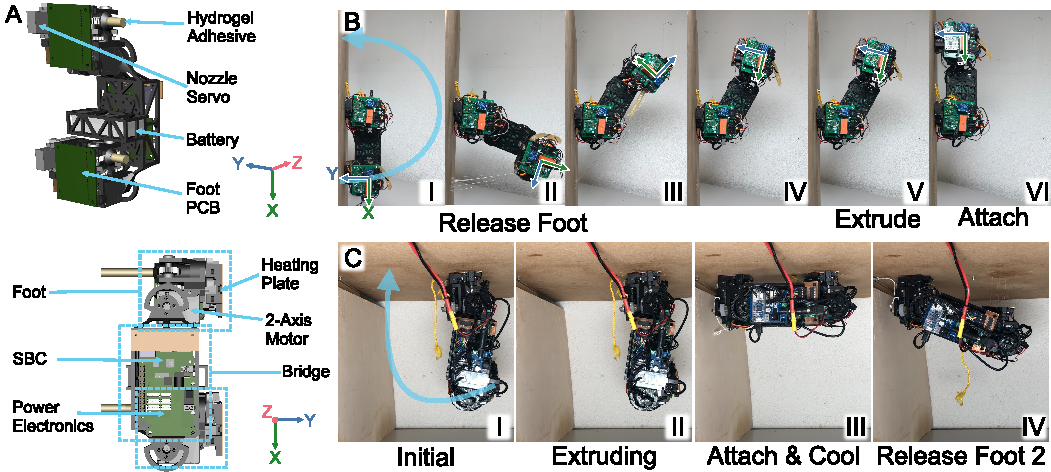
\includegraphics[width=\linewidth]{chapters/papers/SB/figures/fig-6-snailbot-placeholder/fig-6-snailbot-placeholder.pdf}
  \caption{SnailBot: (A) showcases different parts of the robot, (B) demonstrates the robot's ability to scale vertical walls, and (C) inverted, along the ceiling.}
  \label{fig:fig6-placeholder}
\end{figure}

Our proposed climbing robot, SnailBot, uses biodegradable gelatin hydrogel as an adhesive and is fully self-sufficient. While other climbing robots using hot-melt adhesives rely on external power \cite{ROCHAT2011, Wang2013, Osswald2013}, or assume that the environment is covered with the adhesive \cite{Wang2013}, the SnailBot is fully powered through an onboard battery and has an extrusion mechanism to supply fresh adhesive for every step.
% The adhesive has been shown to adhere to various different surfaces, and does not leave any harmful residue; any hydrogel residue left in the environment is biodegradable and water soluble. 

% design choice reasons. (track, etc) => but step most efficient
There are several potential locomotion strategies for climbing robots utilizing biodegradable adhesives. For instance, one could have a rolling track with multiple adhesive elements, or a caterpillar-like locomotion with a prismatic joint shifting the feet. The chosen two-foot rotating design maximizes the distance traveled while minimizing the number of necessary actuators. Since taking a single step can be quite time- and energy-consuming with each heating and cooling cycle, it is important to maximize the distance traveled per step. SnailBot heats the adhesive for 30 seconds, then actively cools it for one minute after pressing. To detatch, the hydrogel is again heated for 30 seconds. With the current chosen parameters for scaling surfaces of any incline, SnailBot manages a speed of 0.59 body lengths/minute or 0.21 cm/s
% 21 cm long).
%detatch 30, extrude + rotate = 20s horiz. or 10s for vertical wall, press 1 minute,

SnailBot consists of three main parts, two feet and a bridge body which connects the two. The two feet are identical to promote modularity. To take steps, SnailBot rotates the bridge and free foot around the fixed foot, out-of-plane to the substrate (Figure~\ref{fig:fig6-placeholder}B,C). See the Supplementary Video S1 for videos of SnailBot climbing vertical and horizontal surfaces.

% why out-of-plane moution, due to shearing. , more load for motor, but less for adhesive. 
An out-of-plane motion for each step was chosen since this minimizes the necessary load on the adhesive. The out-of-plane rotation shifts the center of gravity away from the wall, thus increasing the lever arm and the load for the motor and the maximum necessary torque, when compared with an in-plane rotation. However, the rotational shear resulting from an in-plane rotation is more detrimental to the adhesive properties than the additional forces from the out-of-plane rotation. 

% TODO image
Each foot contains the following components (Figure~\ref{fig:fig7-placeholder}): a dual-axis motor to rotate the foot and extrude the adhesive, a PCB for electrical routing, nozzle and nozzle servo, heating plate upon which the hydrogel is extruded, a heating coil which keeps the hydrogel liquid before extrusion, astick of gelatin-hydrogel adhesive, and for heating and cooling the heating plate a Peltier element, heatsink, and fan. 
A thermocouple near the heating coil in the glue-extrusion system provides closed-loop temperature control. 
The bridge contains the battery, single-board computer which controls everything, and a PCB for power distribution. 
For a detailed list of all components, see the Experimental Section~\ref{subsec:experimental_snailbot}.


\begin{wrapfigure}{r}{0.5\linewidth}
  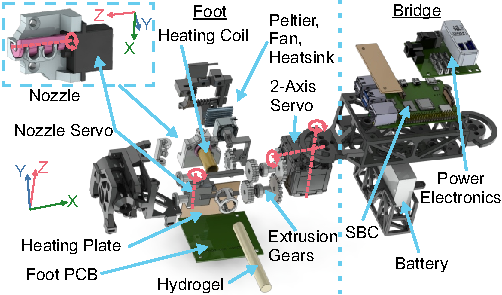
\includegraphics[width=\linewidth]{chapters/papers/SB/figures/fig-7-snailbot-closeup-placeholder/fig-7-snailbot-closeup-placeholder.pdf}
  \caption{SnailBot: exploded view of one foot and the bridge of the climbing robot.}
  \label{fig:fig7-placeholder}
\end{wrapfigure}
% maybe have exploded foot here, or full schematic and mechanism, or robot diagramm with axis

% Adhesive extrusion
% Figure~\ref{fig:fig7-placeholder} shows the adhesive reservoir, a cylinder of hydrogel. Gears on either side are connected to a servo motor which can either push or pull the stick towards the nozzle where the heating coil around a copper tube is located. The gears help with grip, since the hydrogel is visoelastic and would buckle if pushed from the end.

% major challenge: extrusion of glue and spreading of glue on plate. => use gravity with alignment of foot during extrusion. 
Since the gelatin hydrogel is viscoelastic, and then liquid and sticky when heated, extruding the adhesive consistently and evenly is a major challenge. Figure~\ref{fig:fig7-placeholder} top left shows the nozzle and the adhesive reservoir, a cylinder of hydrogel (22.44g). The hydrogel cylinder is fed in from the rear, driven by the servo-powered gears, which push or pull it towards the nozzle, where the heating coil around the copper tube then proceeds to melt it. The gears help with grip, since the hydrogel is visoelastic and would buckle if pushed from the end. The channel then tapers on the top to prevent air accumulation and ensure continuous flow without bubbles. A rotating nozzle flap actuated by the additional servo ensures precise extrusion of glue. This servo is necessary to prevent the back-flow of air into the chamber, and to prevent leakage and continuous dripping of glue. This ensures more accurate extrusion than solely relying on the retraction and advancing of the gluestick to start and stop the flow, such as used in conventional hot-glue guns. A dual nozzle extrusion was used to increase horizontal spread of the glue across the heating plate. Additionally, the nozzle is located towards the top of the rectangular heating plate, and the foot is oriented so that gravity helps the glue spread across the surface of the plate. Depending on the robot orientation this requires the foot to be rotated so that it is aligned differently and with a slight angle to gravity to prevent dripping (Figure~\ref{fig:fig6-placeholder}B-V and C-II). Underneath the heating plate is the Peltier element which provides cooling during attachment with the aid of a heatsink and fan to facilitate adhesion.


% Each foot has one dual-axis motor, where one output is used to rotate the foot and the other is used to drive the gears for extruding the hydrogel. An additional servo is used for actuating the nozzle.
Excluding the hydrogel extrusion, the robot has effectively two degrees of freedom, a rotation around the fixed ankle joint, and one around the moving foot to orient it. The robot can thus take steps and also overcome obstacles of a certain height; however making turns to the left or right would require an additional actuator. 

Figure~\ref{fig:fig6-placeholder}B, C showcases the SnailBot taking a step on a vertical wall and ceiling respectively. In Figure~\ref{fig:fig6-placeholder}B the rear (bottom) foot begins the heating cycle on the heating plate to release the adhesive on that foot. Once the hydrogel has reached the desired temperature, the rear foot is simultaneously raised and rotated, releasing the foot from the substrate. Both the ankle joint in the front foot and the rear foot continue to rotate, until the rear foot is above the front foot and heating plate of the rear foot is again facing the substrate. This is the starting configuration for Figure~\ref{fig:fig6-placeholder}C. Then, the adhesive in the rear foot is extruded (Figure~\ref{fig:fig6-placeholder}B-V and C-II) from the reservoir behind the nozzle that is kept at temperature by the heating coil and thermocouple. Using the motor from the opposite foot, the formerly rear foot is pressed against the substrate while the Peltier element begins cooling to complete the adhesion process. For the next step, the process is repeated with opposite feet (Figure~\ref{fig:fig6-placeholder}C-IV).

%% Would be very interesting to show powerconsumption per step (ideally each stage time + energy)

%Vertical, horizontal, normal climbing
Climbing different surface inclinations results in different loads on the adhesive.
The easiest is 0\degree\, inclination, walking on a flat surface, since gravity already keeps the robot on top of the surface. Increasing elevations increases the shear force, until the robot is climbing a vertical wall (Figure~\ref{fig:fig6-placeholder}B). This is the most challenging scenario for the adhesive since it is weakest in shear and strongest against fully normal forces. Further increasing inclinations results in decreasing shear forces until the robot is hanging from the ceiling (Figure~\ref{fig:fig6-placeholder}C), where the force on the adhesive is fully normal, but the adhesive has to sustain the full weight of the robot (935g). 

\section{Conclusion}
In this work we have shown the feasibility and utility of gelatin-based hydrogels as adhesives for robotic monitoring tasks.
We have characterized the parameters needed to dimension the gelatin-hydrogel as an adhesive, and showcased the adhesion to different substrates with varying surface roughnesses. Finally, we demonstrated the applicability of utilizing a gelatin-hydrogel as a biodegradable adhesive for three robotic environmental monitoring tasks: sensor placement using a UAV, a perching UAV, and a climbing robot. The hydrogel has strong adhesive capabilities, during the characterization we show that only 0.1g or 6x6 mm of a 2mm sheet of the hydrogel can already sustain more than 4kg of pull-off force. Compared with other adhesion methods which work exclusively on certain types of substrates and surface roughnesses, the gelatin-hydrogel maintains at least 2.5kg of pull-off force across all different surfaces, including tree bark, bricks, MDF, glass, and sandpaper of different grit. Since the gelatin-hydrogel is not only water-soluble, but also nontoxic, biocompatible, biodegradable, and even edible, it is ideally suited for situations and environments where leaving potentially toxic and non-biodegradable residue is problematic, such as forest environments for biodiversity or environmental monitoring, and  industrial inspection or infrastructure monitoring. 

Despite the range of surfaces roughnesses tested, wet surfaces can be problematic due to the water solubility of the hydrogel. While water solubility presents an advantage of the solution in terms of residue removal and environmental impact, it is also a limitation on potential application scenarios. Currently, the solution cannot be deployed in wet and humid environments, such an rainforests, since the adhesive would dissolve. The addition of cross-linking polymers to the gelatin \cite{Stoessel2015, Gomez-Estaca2011, Wang2020} during manufacture can increase water resistance, however, the resulting residue should either still be biodegradable and be left to decompose or another method for removal must be developed.

% limitations
% - cooling time, water solubility (rainforest)
For specific applications, the attachment method can be improved to increase adhesion. All demonstrations, perching, climbing robot and sensor placement, employ a rigid copper plate as the interface between adhesive and substrate. As the tests (Figure~\ref{fig:fig3-placeholder}A) show, when the element is used on curved surfaces such as the tree branch, there in lower adhesion due to the reduced surface contact. In such cases, especially with thinner branches and a larger curvature, an adaptive end-effector should be used, which conforms to the surface and maximizes the surface contact. Similarly in nature, animals which utilize adhesion (for instance molluscs such as snails or slugs) usually have soft bodies which adapt and conform to the surface they are attached to. Future work will investigate how to create a conforming attachment surface with high thermal conductivity to the heating and cooling element, for instance by distributing several smaller heating and cooling elements within a conformable silicone backing.

The long cooling times present another challenge for the gelatin hydrogel in certain use-cases, especially when using a UAV with limited flight time. For example, the perching UAV needed to hover for three minutes to wait for the adhesive to cool. For shorter missions, this wait time might outweigh potential energy savings gained by perching. Possible solutions include more efficient cooling through larger and more efficient Peltier-elements, heatsinks, and fans, or cooling through other means, such as liquid or gas cooling. Expelling compressed gas on the surface could rapidly lower the local temperature behind the adhesive, providing much faster cooling and reducing the wait time. In situations where maximal pull-off force is not needed the wait time can be reduced by choosing a sub-optimal cooling temperature. For instance, for sensor placement after the hydrogel is heated, then cooled for 2 minutes, it needs to be pressed for only a few seconds against the substrate. The heating and cooling can be completed before arrival at the target, reducing total mission time.

% The SnailBot also only has two effective degrees of freedom during a step, for it to be able to turn and navigate more complex surfaces, an additional actuator should be added. 
% more thingsthat can be improved with snailbot?

% due to the conflicting requirements of having a conforming contact plate, while still maintaining high thermal conductivity to the heating/cooling element, which is re

% - conformable plate ie soft animals like snails/mollusks also use the soft body in addition to adhesion to conform to surfaces
%     - significant work needed to implement this, not trivial, but we show that in principle the glue works, but for more robust applications should be changed.

% Future work
% Flights for both the sensor placement and the perching UAV were conducted under manual control, with manual alignment and adjustments. To enhance usability by the end-user and lower the barrier for entry, these processes should be automated. By using the onboard cameras to position the UAV, either only the attachment and detachment can be automated, or the entire perching and sensor placement procedure can be automated. This makes these solutions available to a broader user base, increasing safety and efficiency.



% Experimental section
\section{Experimental Section}
\label{sec:experimental_section}


Each configuration and robot (perching UAV, climbing robot and sensor placement with UAV) requires a different holding force depending on the weight.
A table with the weight breakdown of the different components and configurations, including the weight the glue has to hold for that application, can be seen in Table~\ref{tab:weight}.


% \subsection{Gelatin Hydrogel}
% \label{subsec:experimental_section-gelatin_hydrogel}
% The gelatin hydrogel used in this work follows the same composition as in \cite{Geckeler2023b}, it is composed of 24 weight percent (wt\%) of gelatin powder (mesh 40 and bloom factor 260), 25.3 wt\% glucose, 32.5 wt\% glycerin (E422, 99.7\%), 14.5 wt\% de-ionized water, and 3.6 wt\% citric acid (E330). The ingredients are mixed under heat, then cast into corresponding moulds. For the hydrogel reservoir glue sticks of the climbing robot SnailBot, it is cast into cylindrical tubes, for all other applications into sheets of 2 mm, which are then laser-cut into the corresponding area needed for the specific application. 

% Each configuration and robot (perching UAV, climbing robot and sensor placement with UAV) requires a different holding force depending on the weight.
% A table with the weight breakdown of the different components and configurations, including the weight the glue has to hold for that application, can be seen in Table~\ref{tab:weight}.

%/ table with weight breakdown of the different solutions (perching/sensor attachment + snailbot)
\begin{table}
    \centering
    \caption{Weight of different configurations, with weight needed to be held by the hydrogel.}
    % \begin{tabular}{c|c|c}
      % \begin{tabular}[htbp]{@{}lrr@{}}
      \begin{tabular}[t]{lrr}
        Perching UAV  & Mass(g) & \% Total \\
        \hline
        UAV (no Batt.) & 561.38 & 49 \\ 
        UAV Batt. & 332.86 & 29 \\
        Payload Batt.  & 81.79 & 7\\
        Mechanism  & 170.27 & 15\\ 
        Hydrogel (1x)  & 0.8 & $\approx$ 0\\ 
        \hline
        Total & 1147.10 & 100\\
        Supported & 1147.0 & 100%
    \end{tabular}
    \hfill
    \begin{tabular}[t]{lrr}
        SnailBot  & Mass(g) & \% Total \\
        \hline
        Robot & 808.30 & 86\\
        Battery & 81.79 & 9\\
        Hydrogel Sticks  & 44.88 & 5\\ 
        \hline
        Total & 934.97 & 100   \\
        Supported & 934.97 & 100%
    \end{tabular}
    \hfill
    \begin{tabular}[t]{lrr}
        Sensor Placement  & Mass(g) & \% Total \\
        \hline
        UAV (no Batt.) & 561.38 & 48\\ 
        UAV Batt. & 332.86 & 29\\
        Payload Batt. & 81.79 & 7\\
        Mechanism  & 126.02 & 11\\ 
        Sensor Box  & 63.61 & 5\\
        Hydrogel (1x)  & 0.8 & $\approx$ 0\\ 
        \hline
        Total & 1166.46 & 100\\
        Supported & 64.41 & 6%
    \end{tabular}
    \label{tab:weight}
\end{table}

\subsection{UAV}
% drone used
Flight experiments were conducted with the commercial, off-the-shelf DJI Mavic 3 Classic. Despite not being designed for additional payloads, flight performance is still acceptable when additional weight remains below 300g. Table~\ref{tab:weight} lists the added weights for each of the flight configurations. A commercial off-the-shelf UAV was chosen intentionally, to demonstrate the feasibility of achieving complex robotic tasks (perching and sensor placement) with no custom hardware or optimized controllers. This democratizes access to such tasks, and moves them from only being present in research labs to be available to a wide range of end-users.
Of course, for commercial or frequent usage, a platform which is designed for such tasks would increase performance and flight safety.

% power over E-port 
A separate battery for the payload was used for the perching and sensor payload for modularity and to ease integration onto other UAV platforms. With a little extra integration it is also possible to draw power directly from the UAV, for instance through the E-Port interface available on the DJI Mavic Enterprise series \cite{DJI}, reducing the necessary payload weight by removing the extra battery weight. 

% flight parameters for perching
The cooling phase for the perching UAV lasted for 3 minutes, meaning that the UAV must be relatively stationary, pushing against the substrate for this time. Depending on the desired perching timespan, this can be quite long in terms of battery life; the length and efficiency of cooling can be tweaked and improved through the size of Peltier element, the heatsink, and fan. 

% test-setup
\subsection{Experimental Setup}
The experimental setup in Section~\ref{subsec:gelatin_charac} for hydrogel characterization and adhesion strength test on different surfaces consists mainly of two surfaces, one attached to the workbench, and the other attached to  a motorized vertical Z-axis. The fixed bottom plate has the 14,4\ohm; 10W; 300\degree C resistive heating element (GBR-618-12-10-2) beneath the copper plate. The top copper plate for the hydrogel characterization has active cooling, with a fan blowing air onto the plate. This top plate is attached to the motorized Z-axis via a 5 kg load-cell (TAL220B) which allows measuring of the pressing and pull-off force. The load-cell is connected via a HX711 amplifier to an Ardunio, which logs the data. The motorized Z-Axis of a 3D printer is used for the tests.
For the surface roughness tests in Section~\ref{subsec:surface_tests}, a similar setup to above was used, except that the bottom copper plate is replaced with the material being tested. An integrated peltier element in the top plate provides the heating and cooling.


% different peltier elements + heatsink, fans used. 
% motors + electronics used
%% probably schematic for different mechanisms would be nice 

\subsection{Sensor Attachment Mechanism}
\label{subsec:experimental_sensor_placing}
A 3S 950mAh 35C continuous, 70C peak drain LiPo battery was used to power the payload. A Raspberry Pi Pico W was used to remotely control the system with HTTP over WiFi.
The detachable sensor uses a 3-pin magnetic Pogo connector to transfer power to the heating plate and provide attachment. A 25 x 75 mm copper plate is used as the heating plate, pre-loaded with 0.8g of adhesive (4 x 0.2g), where a 14,4\ohm; 10W; 300\degree C resistive heating element (GBR-618-12-10-2) is used to heat the plate. The 11.1 V nominal voltage of the battery is directly connected to the heating element, and converted to 5V for the Pico microcontroller using a 5V, 3.4A step-down voltage regulator (D30V30F5). The heating element is switched by the Pico using an N-channel MOSFET (IRLRU8743).
The sensor system used for sensor placement with a UAV is based on the TinyDuino platform, with a separate 3.7 V 150 mAh LiPo battery for power. The Combo Sensor Tinyshield was used, with temperature, humidity (Silicon Labs Si7020-A10), barometric pressure (Bosch BMP280), 9-axis IMU (ST LSM9DS1), and ambient light (TAOS TSL2572).

\subsection{UAV Perching Mechanism}
\label{subsec:experimental_perching}
The perching mechanism is powered by the same 3S 950mAh 35C continuous, 70C peak drain LiPo battery, and also controlled by a Raspberry Pi Pico W over WiFi. 
0.8g of adhesive (4 x 0.2g) are placed on the 20 x 53 mm copper heating plate. It is heated and cooled by a thermoelectric Peltier element (CP60233) where excess heat is removed by a 20x20x6mm heatsink (TGH-0200-02) with a 30x30x15mm 12V DC 6 CFM fan (MF30151V1-1000U-A99). This is connected to the body of the payload with a spring-loaded swivel joint, permitting rotation around the UAV's pitch axis. During perching, first the adhesive is heated for 30 s to 60\degree C, then the UAV approaches and maintains contact for three minutes until the cooling cycle is complete. To detach, the adhesive is again heated for 30 s.

Unlike the sensor placement payload, which had passive cooling, the perching payload has both active cooling and heating which results in more electronic components. A DPDT DC 8A relay (RT424012) is used to switch the polarity of the Peltier element to switch between heating and cooling; an N-channel MOSFET (IRLRU8743) is used to switch the fan on or off. The same 5V step-down voltage regulator converts the 11.1V battery voltage to 5V for the microcontroller and another to 9V for the Peltier element (CP60233) using a step down voltage regulator (D36V50F9).

\subsection{SnailBot: Climbing Robot}
\label{subsec:experimental_snailbot}
The climbing robot SnailBot not only has active heating and cooling, but also adhesive extrusion and locomotion, which makes it the most complicated mechanism with the most components. The SnailBot consists of three main parts, two identical feet and a bridge connecting the two. The bridge contains a Raspberry Pi 4 used to process the inputs and control the components, with a Robotis Dynamixel U2D2 Powerboard used to interface the Dynamixel motors with the Pi and battery. The same 3S 950mAh 35C continuous drain LiPo battery is also stored on the bridge. A custom PCB on the bridge has a 5V, 3.4A step-down voltage regulator (D30V30F5) to provide power to the Pi, and an analog to digital converter (ADC, MCP3008-I/P) to enable reading of the K-type thermocouple (AD8495) used for closed loop temperature control.

The current iteration of the SnailBot consists of three actuators in each foot, one of which is for locomotion by rotating the foot, one for extruding the hydrogel, and one for the nozzle. This design was chosen for simplicity and compactness; a single Dynamixel 2XL-430-W250-T servo with two output axis is used for extrusion and foot rotation, and a much smaller 9g servo (DS S006L) is used to control the nozzle. The copper plate comprising the contact surface at the foot is 41x55mm.
In the future, to also allow the SnailBot to rotate and make turns at least one additional actuator should be added on the bridge to allow rotation in the orthogonal direction. The Dynamixel motor wires are directly connected to the bridge. All other components are connected through a custom PCB located on the foot. This PCB connects  similar electrical components as on the perching mechanism, a Peltier element (CP60233), DPDT DC 8A relay (RT424012) for switching the polarity of the Peltier power, MOSFET (IRF540) for triggering the Peltier element, 25x21x3.5mm heatsink (TGH-0210-01), 17x17x3mm fan (ASB01703HA3-00CAH), a 3.3V voltage regulator (D24V22F3) for heating wire, and a 9V step down voltage regulator (D36V50F9) for the Peltier element.  A 5.65 Ohm/m resistance wire wrapped around the copper tube feeding the hydrogel into the nozzle is used to melt and keep it liquid before extrusion. In addition, the SnailBot also has a K-type thermocouple (AD8495) and an analog amplifier,  which enables closed-loop temperature control using a PID controller to keep the hydrogel ready to extrude at 60\degree.


\medskip
\textbf{Supporting Information} \par %Please delete the Suppporting Information statement if it is not applicable. Please supply Supporting Information in another file. Supporting information should not be provided in .tex format
Supporting Information (Supplementary Video S1) is available from the Wiley Online Library or from the author.



% Acknowledgements
\medskip
\textbf{Acknowledgment} \par %delete if not applicable))
This work was supported by the Swiss National Science Foundation through the Eccellenza under Grant number 186865. The authors would also like to thank Biogel AG for graciously providing the gelatin powder.
% 
% References
\medskip

% Use the following code if you wish to generate your bibliography with BibTeX;
% replace the string "MSP-template" below with the name(s) of
% the BibTeX data base(s) you want to use.
% The resulting bibliography-output (the content of the .bbl file)
% must be pasted back into this file before submission.
% Please also include your BibTeX data base file(s) in your submission
% so that we can re-run BibTeX if necessary.
%
\bibliographystyle{MSP}
%\bibliography{MSP-template}
\bibliography{references.bib}

% \textbf{References}\\

% 1	((Journal articles)) a) A. B. Author 1, C. D. Author 2, Adv. Mater. 2006, 18, 1; b) A. Author 1, B. Author 2, Adv. Funct. Mater. 2006, 16, 1.\\
% 2	((Work accepted)) A. B. Author 1, C. D. Author 2, Macromol. Rapid Commun., DOI: 10.1002/marc.DOI.\\
% 3	((Books)) H. R. Allcock, Introduction to Materials Chemistry, Wiley, Hoboken, NJ, USA 2008.\\
% 4	((Edited books or proceedings volumes)) J. W. Grate, G. C. Frye, in Sensors Update, Vol. 2 (Eds: H. Baltes, W. Göpel, J. Hesse), Wiley-VCH, Weinheim, Germany 1996, Ch. 2.\\
% 5	((Presentation at a conference, proceeding not published)) Author, presented at Abbrev. Conf. Title, Location of Conference, Date of Conference ((Month, Year)).\\
% 6	((Thesis)) Author, Degree Thesis, University (location if not obvious), Month, Year.\\
% 7	((Patents)) a) A. B. Author 1, C. D. Author 2 (Company), Country Patent Number, Year; b) W. Lehmann, H. Rinke (Bayer AG) Ger. 838217, 1952.\\
% 8	((Website)) Author, Short description or title, URL, accessed: Month, Year.\\
% 9	…((Please include all authors, and do not use “et al.”))\\




% Figures/tables and captions
% Permission statements are required for all figures reproduced or adapted from previously published articles/sources. Please also ensure that all necessary permissions to reproduce images have been received
% Please remove these statements for original figures


% \begin{figure}
%   \includegraphics[width=\linewidth]{placeholder-image.png}
%   \caption{Figure 1 caption goes here. Reproduced with permission.\textsuperscript{[Ref.]} Copyright Year, Publisher. }
%   \label{fig:boat1}
% \end{figure}

% \begin{table}
%  \caption{Table 1 caption}
%   \begin{tabular}[htbp]{@{}lll@{}}
%     \hline
%     Description 1 & Description 2 & Description 3 \\
%     \hline
%     Row 1, Col 1  & Row 1, Col 2  & Row 1, Col 3  \\
%     Row 2, Col 1  & Row 2, Col 2  & Row 2, Col 3  \\
%     \hline
%   \end{tabular}
% \end{table}


% Table of contents entry should be 50 - 60 words long
% Image should be 55 mm broad and 50 mm high or 110 mm broad and 20 mm high


\begin{figure}
\textbf{Table of Contents}\\
\medskip
  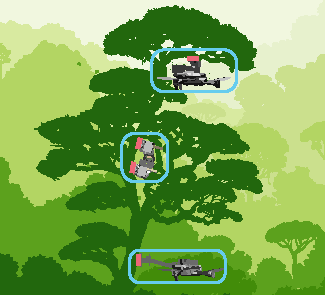
\includegraphics{figures/toc/toc.pdf}
  \medskip
  \caption*{Gelatin-based hydrogels are presented as a robust, biodegradable, and water-soluble method of adhesion for robotic environmental monitoring. Factors affecting the adhesion strength are characterized, and the hydrogel is tested on different materials with varying surface roughness. The utility of the hydrogel is showcased for three environmental monitoring tasks: a perching UAV, a climbing robot, and sensor placement.}
\end{figure}


\end{document}
